%% \documentclass[handout,t]{beamer} % HANDOUT
%% \documentclass[handout,notes=show,t]{beamer} % NOTES
\documentclass[t]{beamer} % SLIDES
\usepackage{etex}

\usetheme{DSM}
\usepackage{beamer-tools-dsm}

\input{lib/math}  % basic mathematical notation
\input{lib/text}  % some useful macros for plain text
\input{lib/stat}  % notation for probability theory and statistics
\input{lib/vector}% convenience macros for vectors and matrices

%%%
%%% local configuration adjustments
%%%

%%% You can change pre-defined colours here, override built-in macros from the
%%% style definition and standard library, as well as define macros needed by
%%% all local documents.

%%% e.g. adjust counterpoint (dark green) for data projectors where greens are
%%% far too bright, as well as green component of light colour and pure green
%%% (of course, it's a better solution to adjust the gamma settings of your monitor)
%%
%% \definecolor{counterpoint}{rgb}{.1, .3, 0}
%% \definecolor{light}{rgb}{.45, .3, .55}
%% \definecolor{puregreen}{rgb}{0, .35, 0}

%% ----- extra packages we need to load

\usepackage{tikz}
\usepackage{alltt}              % code examples with nicely formatted comments
\usepackage{hieroglf}           % hieroglyph font for the archeology example
\usepackage{rotating}
\usepackage{multirow}

\usetikzlibrary{arrows.meta}
\usetikzlibrary{shadows}

%% ----- predefined TikZ styles

%% diagram:
%%   box[=colour]   ... shaded text box with drop shadow
%%   arrow[=colour] ... thick arrow between boxes
%%   ghost          ... invisible box (white)
\tikzstyle{diagram box}[secondary]=[
rectangle, rounded corners=1ex, inner sep=5pt, minimum height=4ex, minimum width=4ex,
thick, draw=#1, top color=#1!5!white, bottom color=#1!25!white, drop shadow]

\tikzstyle{diagram ghost}=[
rectangle, rounded corners=1ex, inner sep=5pt, minimum height=4ex, minimum width=4ex,
thick, draw=white, color=white]

\tikzstyle{diagram arrow}[secondary]=[
->, >={Latex[width=4pt, length=4pt]}, ultra thick, color=#1]


%% ----- general copyright message (authors may change between versions of the tutorial)
\newcommand{\dsmcopyright}{%
  Copyright \textcopyright\ 2009--2016 Evert, Lenci, Baroni \& Lapesa | 
  Licensed under CC-by-sa version 3.0}


%% ----- automatically show TOC reminder at beginning of each subsection
\AtBeginSubsection[]
{
  \begin{frame}
    \frametitle{Outline}
    \tableofcontents[current,currentsubsection]
  \end{frame}
}

%% ----- some useful macros for the SIGIL course

%% \begin{Rcode} .. \end{Rcode}
\newenvironment{Rcode}[1][]{%
\setbeamercolor{block title}{fg=counterpoint,bg=counterpoint!15!white}%
\setbeamercolor{block body}{bg=counterpoint!5!white}\small%
\begin{block}{#1}\begin{alltt}\ungap[1]}{%
\ungap[1]\end{alltt}\end{block}}

%% > plot(x,y)      \REM{this produces a scatterplot}
\newcommand{\REM}[2][\small]{\textsf{#1\color{primary}\# #2}}

%% nice colour for R output: \begin{Rout} .. \end{Rout}
\newenvironment{Rout}[1][\footnotesize]{%
  \begin{footnotesize}#1\color{secondary}\bfseries}{%
  \color{black}\mdseries\end{footnotesize}}

%% symbols for centroid vector and singular value matrix 
%% \newcommand{\vmu}[1][]{\boldsymbol{\mu}\ifthenelse{\equal{#1}{}}{}{^{(#1)}}}
\newcommand{\Msigma}{\boldsymbol{\Sigma}}

%% rotated column labels for table (to fit long text into narrow columns
\newcommand{\rotLabel}[2][60]{\begin{rotate}{#1}#2\end{rotate}}

 % local adjustments to configuration and macros

%%%%%%%%%%%%%%%%%%%%%%%%%%%%%%%%%%%%%%%%%%%%%%%%%%%%%%%%%%%%%%%%%%%%%%
%% Titlepage

\title[DSM Tutorial -- Part 2]{Distributional Semantic Models}
\subtitle{Part 2: The parameters of a DSM}
\author[\textcopyright\ Evert/Lenci/Baroni/Lapesa]{%
  Stefan Evert\inst{1}\\
  {\footnotesize with  Alessandro Lenci\inst{2}, Marco Baroni\inst{3} and Gabriella Lapesa\inst{4}}}
\institute[CC-by-sa]{%
  \inst{1}Friedrich-Alexander-Universität Erlangen-Nürnberg, Germany\\
  \inst{2}University of Pisa, Italy\\
  \inst{3}University of Trento, Italy\\
  \inst{4}University of Stuttgart, Germany
}

\date[wordspace.collocations.de]{
  \href{http://wordspace.collocations.de/doku.php/course:start}{\primary{\small http://wordspace.collocations.de/doku.php/course:start}}\\
  \light{\tiny \dsmcopyright}}

\begin{document}

\showLogo
\frame{\titlepage}
\hideLogo

%%%%%%%%%%%%%%%%%%%%%%%%%%%%%%%%%%%%%%%%%%%%%%%%%%%%%%%%%%%%%%%%%%%%%%

\section*{Outline}
\frame{ 
  \frametitle{Outline}
  \tableofcontents
}

%%%%%%%%%%%%%%%%%%%%%%%%%%%%%%%%%%%%%%%%%%%%%%%%%%%%%%%%%%%%%%%%%%%%%%
\section{DSM parameters}

\begin{frame}
  \frametitle{General definition of DSMs}
  % \framesubtitle{}

  \ungap
  \begin{block}{}
    A \h{distributional semantic model} (DSM) is a scaled and/or
    transformed co-occurrence matrix $\mathbf{M}$, such that each row $\vx$
    represents the distribution of a target term across contexts.
  \end{block}

  \begin{center}
    \begin{small}
      \setlength{\arrayrulewidth}{1pt}
      \begin{tabular}{r*{6}{|c}|}
        & get & see & use & hear & eat & kill \\
        \hline
        knife &  0.027 & -0.024 &  0.206 & -0.022 & -0.044 & -0.042 \\
        \hline
        cat   &  0.031 &  0.143 & -0.243 & -0.015 & -0.009 &  0.131 \\
        \hline
        \primary{dog}   & \primary{-0.026} &  \primary{0.021} & \primary{-0.212} &  \primary{0.064} &  \primary{0.013} &  \primary{0.014} \\
        \hline
        boat  & -0.022 &  0.009 & -0.044 & -0.040 & -0.074 & -0.042 \\
        \hline
        cup   & -0.014 & -0.173 & -0.249 & -0.099 & -0.119 & -0.042 \\
        \hline
        pig   & -0.069 &  0.094 & -0.158 &  0.000 &  0.094 &  0.265 \\
        \hline
        banana&  0.047 & -0.139 & -0.104 & -0.022 &  0.267 & -0.042 \\
        \hline
      \end{tabular}
    \end{small}
  \end{center}

  \hh{Term} = word, lemma, phrase, morpheme, word pair, \ldots
\end{frame}

\begin{frame}
  \frametitle{General definition of DSMs}
  % \framesubtitle{}

  Mathematical notation:
  \begin{itemize}
  \item $k \times n$ co-occurrence matrix $\mathbf{M}\in \setR^{k\times n}$ (example: $7\times 6$)
    \begin{itemize}
    \item $k$ rows = \h{target} terms 
    \item $n$ columns = \h{features} or \hh{dimensions}
    \end{itemize}
    \begin{small}
      \gap[.5]
      \[
      \mathbf{M} =
      \begin{bmatrix}
        m_{11} & m_{12} & \cdots & m_{1n} \\
        m_{21} & m_{22} & \cdots & m_{2n} \\
        \vdots & \vdots & & \vdots \\
        m_{k1} & m_{k2} & \cdots & m_{kn}
      \end{bmatrix}
      \]
    \end{small}
  \item distribution vector $\Vector{m}_i$ = $i$-th row of $\mathbf{M}$, e.g.\ $\Vector{m}_3 = \Vector{m}_{\text{dog}} \in \setR^n$
  \item components $\Vector{m}_i = (m_{i1}, m_{i2}, \ldots, m_{in})$ = features of $i$-th term:
    \begin{align*}
      \Vector{m}_3 &= (-0.026, 0.021, -0.212, 0.064, 0.013, 0.014) \\
      &= (m_{31}, m_{32}, m_{33}, m_{34}, m_{35}, m_{36})
    \end{align*}
  \end{itemize}

\end{frame}


%%%%%%%%%%%%%%%%%%%%%%%%%%%%%%%%%%%%%%%%%%
\subsection{A taxonomy of DSM parameters}

\begin{frame}<beamer:1| handout:1>[label=DSM_parameters]
  \frametitle{Overview of DSM parameters}
  
  \footnotesize\centering
  \begin{tikzpicture}
    \node[diagram box=black] (corpus) at (0, 6.5) {pre-processed corpus with linguistic annotation} ;
    \visible<beamer:1,3-| handout:1,3->{
      \node[diagram box] (tt_terms) at (+3, 5) {define target \& feature terms} ;
      \node[diagram box] (tc_terms) at (-3, 5) {define target terms} ; 
    }
    \visible<beamer:2| handout:2>{
      \node[diagram dark box=primary] (tt_terms) at (+3, 5) {define target \& feature terms} ;
      \node[diagram dark box=primary] (tc_terms) at (-3, 5) {define target terms} ; 
    }
    \visible<beamer:1-2,4-| handout:1-2,4->{
      \node[diagram box] (tt_span) at (+3, 4) {type \& size of co-occurrence} ;
    }
    \visible<beamer:3| handout:3>{
      \node[diagram dark box=primary] (tt_span) at (+3, 4) {type \& size of co-occurrence} ;
    }
    \visible<beamer:1-3,5-| handout:1-3,5->{
      \node[diagram box] (tc_context) at (-3, 4) {context tokens or types} ;
    }
    \visible<beamer:4| handout:4>{
      \node[diagram dark box=primary] (tc_context) at (-3, 4) {context tokens or types} ;
    }
    \visible<beamer:1-4,6-| handout:1-4,6->{
      \node[diagram box=black] (geom_prob) at (0, 3) {$\mathbf{M}$} ;
    }
    \visible<beamer:5| handout:5>{
      \node[diagram dark box=primary] (geom_prob) at (0, 3) {$\mathbf{M}$} ;
    }
    \node[diagram ghost] (prob) at (2, 2) {} ;
    \visible<beamer:1-5,7-| handout:1-5,7->{
      \node[diagram box] (scoring) at (-2, 2) {feature scaling} ;
    }
    \visible<beamer:6| handout:6>{
      \node[diagram dark box=primary] (scoring) at (-2, 2) {feature scaling} ;
    }
    \visible<beamer:1-6,8-| handout:1-6,8->{
      \node[diagram box] (metric) at (-2, 1) {similarity/distance measure + normalization} ;
    }
    \visible<beamer:7| handout:7>{
      \node[diagram dark box=primary] (metric) at (-2, 1) {similarity/distance measure + normalization} ;
    }
    \visible<beamer:1-7,9-| handout:1-7,9->{
      \node[diagram box] (dimred) at (-2, 0) {dimensionality reduction} ;
    }
    \visible<beamer:8| handout:8>{
      \node[diagram dark box=primary] (dimred) at (-2, 0) {dimensionality reduction} ;
    }
    \draw[diagram arrow=counterpoint] (corpus) -- node[right=1.5em] {term-term matrix} (tt_terms) ;
    \draw[diagram arrow] (tt_terms) -- (tt_span) ;
    \draw[diagram arrow] (tt_span) -- (geom_prob) ;
    \draw[diagram arrow=counterpoint] (corpus) -- node[left=1.5em] {term-context matrix} (tc_terms) ;
    \draw[diagram arrow] (tc_terms) -- (tc_context) ;
    \draw[diagram arrow] (tc_context) -- (geom_prob) ;
    \draw[diagram arrow=counterpoint] (geom_prob) -- node[right=1.5em] (probanal) {probabilistic analysis} (prob) ;
    \node[below=1mm of probanal, text width=30mm, align=center, color=counterpoint] {embedding learned by\\ neural network} ;
    \draw[diagram arrow=counterpoint] (geom_prob) -- node[left=1.5em] {geometric analysis} (scoring) ;
    \draw[diagram arrow] (scoring) -- (metric) ;
    \draw[diagram arrow] (metric) -- (dimred) ;
  \end{tikzpicture}
\end{frame}


\begin{frame}[fragile]
  \frametitle{Term-context matrix}
  % \framesubtitle{}

  \h{Term-context matrix} records frequency of term in each individual context (e.g.\ sentence, document, Web page, encyclopaedia article)
  
  \gap[2]
  \begin{center}
  \(
  \mathbf{F} = 
  \begin{bmatrix}
    \cdots & \vf_1 & \cdots \\
    \cdots & \vf_2 & \cdots \\
    & \vdots & \\
    & \vdots & \\
    \cdots & \vf_k & \cdots \\
  \end{bmatrix}
  \)
  \hspace{5mm}
  \begin{small}
    \setlength{\arrayrulewidth}{1pt}
    \begin{tabular}[c]{r*{7}{|c}|}
      \multicolumn{1}{c}{}
      & \multicolumn{1}{c}{\rotLabel{Felidae}}
      & \multicolumn{1}{c}{\rotLabel{Pet}}
      & \multicolumn{1}{c}{\rotLabel{Feral}}
      & \multicolumn{1}{c}{\rotLabel{Bloat}}
      & \multicolumn{1}{c}{\rotLabel{Philosophy}}
      & \multicolumn{1}{c}{\rotLabel{Kant}}
      & \multicolumn{1}{c}{\rotLabel{Back pain}} \\
      \cline{2-8}
      cat      &      10 &  10 &     7 &    -- &         -- &   -- &        -- \\
      \cline{2-8}
      dog      &      -- &  10 &     4 &    11 &         -- &   -- &        -- \\
      \cline{2-8}
      animal   &       2 &  15 &    10 &     2 &         -- &   -- &        -- \\
      \cline{2-8}
      time     &       1 &  -- &    -- &    -- &          2 &    1 &        -- \\
      \cline{2-8}
      reason   &      -- &   1 &    -- &    -- &          1 &    4 &         1 \\
      \cline{2-8}
      cause    &      -- &  -- &    -- &     2 &          1 &    2 &         6 \\
      \cline{2-8}
      effect   &      -- &  -- &    -- &     1 &         -- &    1 &        -- \\
      \cline{2-8}
    \end{tabular}
  \end{small}
  \end{center}

\begin{Rcode}
> TC <- DSM_TermContext
> head(TC, Inf) \REM{extract full co-oc matrix from DSM object}
\end{Rcode}
\end{frame}

\begin{frame}[fragile]
  \frametitle{Term-term matrix}
  % \framesubtitle{}

  \h{Term-term matrix} records co-occurrence frequencies with feature terms for each target term 

  \gap[2]
  \begin{center}
  \(
  \mathbf{M} = 
  \begin{bmatrix}
    \cdots & \vm_1 & \cdots \\
    \cdots & \vm_2 & \cdots \\
    & \vdots & \\
    & \vdots & \\
    \cdots & \vm_k & \cdots \\
  \end{bmatrix}
  \)
  \hspace{3mm}
  \begin{small}
    \setlength{\arrayrulewidth}{1pt}
    \begin{tabular}[c]{r|c@{$\;$}*{6}{|@{$\;$}c@{$\;$}}|}
      \multicolumn{1}{c}{}
      & \multicolumn{1}{c}{\rotLabel{breed}}
      & \multicolumn{1}{c}{\rotLabel{tail}}
      & \multicolumn{1}{c}{\rotLabel{feed}}
      & \multicolumn{1}{c}{\rotLabel{kill}}
      & \multicolumn{1}{c}{\rotLabel{important}}
      & \multicolumn{1}{c}{\rotLabel{explain}}
      & \multicolumn{1}{c}{\rotLabel{likely}} \\
      \cline{2-8}
      cat     &  83 &  17 &   7 &  37 &  -- &   1 &  -- \\
      \cline{2-8}
      dog     & 561 &  13 &  30 &  60 &   1 &   2 &   4 \\
      \cline{2-8}
      animal  &  42 &  10 & 109 & 134 &  13 &   5 &   5 \\
      \cline{2-8}
      time    &  19 &   9 &  29 & 117 &  81 &  34 & 109 \\
      \cline{2-8}
      reason  &   1 &  -- &   2 &  14 &  68 & 140 &  47 \\
      \cline{2-8}
      cause   &  -- &   1 &  -- &   4 &  55 &  34 &  55 \\
      \cline{2-8}
      effect  &  -- &  -- &   1 &   6 &  60 &  35 &  17 \\
      \cline{2-8}
    \end{tabular}
  \end{small}
  \end{center}

\begin{Rcode}
> TT <- DSM_TermTerm
> head(TT, Inf)
\end{Rcode}
\end{frame}

\begin{frame}
  \frametitle{Term-term matrix}
  % \Framesubtitle{}

  Some footnotes:
  \begin{itemize}
  \item Often target terms $\neq$ feature terms
    \begin{itemize}
    \item e.g.\ nouns described by co-occurrences with verbs as features
    \item identical sets of target \& feature terms \so symmetric matrix
    \end{itemize}
  \item Different types of co-occurrence \citep{Evert:08}
    \begin{itemize}
    \item \hh{surface context} (word or character window)
    \item \hh{textual context} (non-overlapping segments)
    \item \hh{syntactic context} (dependency relation)
    \end{itemize}
  \item Can be seen as smoothing of term-context matrix
    \begin{itemize}
    \item average over similar contexts (with same context terms)
    \item data sparseness reduced, except for small windows
    \item we will take a closer look at the relation between term-context and term-term models in part 5 of this tutorial
    \end{itemize}
  \end{itemize}

\end{frame}

%%%%%%%%%%%%%%%%%%%%%%%%%%%%%%%%%%%%%%%%%%%%%%%%%%%%%%%%%%%%%%%%%%%%%%
\againframe<beamer:2| handout:2>{DSM_parameters}

\begin{frame}
  \frametitle{Definition of target and feature terms}

  \ungap
  \begin{itemize}
  \item Choice of linguistic unit
    \begin{itemize}
    \item words
    \item bigrams, trigrams, \ldots
    \item multiword units, named entities, phrases, \ldots
    \item morphemes
    \item word pairs (\hand\ analogy tasks)
    \end{itemize}
  \item<2-> Linguistic annotation
    \begin{itemize}
    \item word forms (minimally requires tokenisation)
    \item often lemmatisation or stemming to reduce data sparseness:\\
      \emph{go, goes, went, gone, going} \so \emph{go}
    \item POS disambiguation (\emph{light}/N \vs\ \emph{light}/A \vs\ \emph{light}/V)
    \item word sense disambiguation (\emph{bank}\tsub{river} \vs\ \emph{bank}\tsub{finance})
    \item abstraction: POS tags (or bigrams) as feature terms
    \end{itemize}
  \item<3-> Trade-off between deeper linguistic analysis and
    \begin{itemize}
    \item need for language-specific resources
    \item possible errors introduced at each stage of the analysis
    \end{itemize}
  \end{itemize}
\end{frame}

\begin{frame}
  \frametitle{Effects of linguistic annotation}
  \framesubtitle{}

  \centering
  Nearest neighbours of \emph{walk} (BNC)
  \ungap\footnotesize
  \begin{columns}[t]
    \column{4cm}
    \begin{block}{word forms}
      \begin{itemize}
      \item stroll
      \item \counterpoint{walking}
      \item \counterpoint{walked}
      \item go
      \item path
      \item drive
      \item ride
      \item wander
      \item sprinted
      \item sauntered
      \end{itemize}
    \end{block}
    \column{4cm}
    \begin{block}{lemmatised + POS}
      \begin{itemize}
      \item hurry
      \item stroll
      \item stride
      \item trudge
      \item amble
      \item wander
      \item \primary{walk} \secondary{(noun)}
      \item \counterpoint{walking}
      \item retrace
      \item scuttle 
      \end{itemize}
    \end{block}
  \end{columns}

  \hfill\light{\tiny \url{http://clic.cimec.unitn.it/infomap-query/}}
  \addnote{All models built with Infomap NLP: 2-word window, 20k targets, 2k features, 300 latent dims}%
  \addnote{Lemmatised model uses BNC lemma annotation (with POS category)}%
\end{frame}

\begin{frame}
  \frametitle{Effects of linguistic annotation}

  \centering
  Nearest neighbours of \emph{arrivare} (Repubblica)
  \ungap\footnotesize
  \begin{columns}[t]
    \column{4cm}
    \begin{block}{word forms}
      \begin{itemize}
      \item  giungere
      \item  \counterpoint{raggiungere}
      \item  \primary{arrivi}
      \item  raggiungimento
      \item  \counterpoint{raggiunto}
      \item  trovare
      \item  \counterpoint{raggiunge}
      \item  \primary{arrivasse}
      \item  \primary{arriver\`a}
      \item  concludere
      \end{itemize}
    \end{block}
    \column{4cm}
    \begin{block}{lemmatised + POS}
      \begin{itemize}
      \item giungere
      \item aspettare
      \item attendere
      \item arrivo \secondary{(noun)}
      \item ricevere
      \item accontentare
      \item approdare
      \item pervenire
      \item venire
      \item piombare
      \end{itemize}
    \end{block}
  \end{columns}
  
  \hfill\light{\tiny \url{http://clic.cimec.unitn.it/infomap-query/}}
  \addnote{Colours seem to indicate inflected forms belonging to the same lemma.}%
  \addnote{Based on La Repubblica SSLMiT corpus}%
  \addnote{Lemmatised model includes two-letter POS codes}%
\end{frame}

\begin{frame}
  \frametitle{Selection of target and feature terms}
  
  \begin{itemize}
  \item Full-vocabulary models are often unmanageable
    \begin{itemize}
    \item 762,424 distinct word forms in BNC, 605,910 lemmata
    \item large Web corpora have $>$ 10 million distinct word forms
    \item low-frequency targets (and features) do not provide reliable distributional information (too much ``noise'')
    \end{itemize}
  \item<2-> Frequency-based selection
    \begin{itemize}
    \item minimum corpus frequency: $f \geq F_{\min}$
    \item or accept $n_w$ most frequent terms
    \item sometimes also upper threshold: $F_{\min}\leq f\leq F_{\max}$
    \end{itemize}
  \item<3-> Relevance-based selection
    \begin{itemize}
    \item criterion from IR: document frequency $df$
    \item terms with high $df$ are too general \so uninformative
    \item terms with very low $df$ may be too sparse to be useful
    \end{itemize}
  \item<4-> Other criteria
    \begin{itemize}
    \item POS-based filter: no function words, only verbs, \ldots
    \end{itemize}
  \end{itemize}
\end{frame}

%%%%%%%%%%%%%%%%%%%%%%%%%%%%%%%%%%%%%%%%%%%%%%%%%%%%%%%%%%%%%%%%%%%%%%
\againframe<beamer:3| handout:3>{DSM_parameters}

\begin{frame}
  \frametitle{Surface context}
  
  \begin{center}
    Context term occurs \primary{within a span of $k$ words} around target.
  \end{center}

  The \secondary{\uline{silhouette of the}}\primary{\dotuline{ sun }}\secondary{\uline{beyond a wide-open}} bay on \secondary{\uline{the lake; the}}\primary{\dotuline{ sun }}\secondary{\uline{still glitters although}} evening has arrived in Kuhmo. It's midsummer; the living room has its instruments and other objects in each of its corners.
  $\quad$ \primary{[L3/R3 span, $k = 6$]}
  
  \gap
  Parameters:
  \begin{itemize}
  \item span size (in words or characters)
  \item symmetric \vs\ one-sided span
  \item uniform or ``triangular'' (distance-based) weighting
  \item spans clamped to sentences or other textual units?
  \end{itemize}
\end{frame}


\begin{frame}
  \frametitle{Effect of span size}
  \framesubtitle{}

  \centering
  Nearest neighbours of \emph{dog} (BNC)
  \ungap\footnotesize
  \begin{columns}[t]
    \column{4cm}
    \begin{block}{2-word span}
      \begin{itemize}
      \item cat
      \item horse
      \item fox
      \item \counterpoint{pet}
      \item rabbit
      \item pig
      \item \counterpoint{animal}
      \item mongrel
      \item sheep
      \item pigeon
      \end{itemize}
    \end{block}
    \column{4cm}
    \begin{block}{30-word span}
      \begin{itemize}
      \item \primary{kennel}
      \item puppy
      \item \counterpoint{pet}
      \item bitch
      \item \counterpoint{terrier}
      \item \counterpoint{rottweiler}
      \item \counterpoint{canine}
      \item cat
      \item \primary{to bark}
      \item \counterpoint{Alsatian}
      \end{itemize}
    \end{block}
  \end{columns}

  \hfill\light{\tiny \url{http://clic.cimec.unitn.it/infomap-query/}}
\end{frame}


\begin{frame}
  \frametitle{Textual context}
  
  \begin{center}
    Context term is in the \primary{same linguistic unit} as target.
  \end{center}

  {\color{secondary}The silhouette of the} \primary{sun}
  {\color{secondary}beyond a wide-open bay on the lake; the}
  \primary{sun} {\color{secondary}still glitters although evening has
    arrived in Kuhmo.} It's midsummer; the living room has its
  instruments and other objects in each of its corners.
  
  \gap
  Parameters:
  \begin{itemize}
  \item type of linguistic unit
    \begin{itemize}
    \item sentence
    \item paragraph
    \item turn in a conversation
    \item Web page
    \end{itemize}
  \end{itemize}
\end{frame}

\begin{frame}
  \frametitle{Syntactic context}
  
  \ungap
  \begin{center}
    Context term is linked to target by a \primary{syntactic dependency}\\
    (e.g. subject, modifier, \ldots).
  \end{center}

  The  \tikz[remember picture, inner sep=0pt, text depth=0pt]{\node (silhouette) {\secondary{silhouette}}}
  of the \tikz[remember picture, inner sep=0pt, text depth=0pt, text height=1.5ex]{\node (sun1) {\primary{sun}}} beyond a
  wide-open \tikz[remember picture, inner sep=0pt, text depth=0pt]{\node (bay) {\secondary{bay}}}
  on the lake; the \tikz[remember picture, inner sep=0pt, text depth=0pt, text height=1.5ex]{\node (sun2) {\primary{sun}}}
  still \tikz[remember picture, inner sep=0pt, text depth=0pt]{\node (glitters) {\secondary{glitters}}}
  although evening has arrived in Kuhmo. It's midsummer; the living room has its instruments 
  and other objects in each of its corners.
  
  \gap
  Parameters:
  \begin{tikzpicture}[remember picture, overlay]
    \draw[->, >={Latex}, secondary, thick] (silhouette.north east) to[out=45, in=135] (sun1.north west)  ;
    \draw[->, >={Latex}, secondary, thick] (sun1.north east) to[out=20, in=160] (bay.north west)  ;
    \draw[<-, >={Latex}, secondary, thick] (sun2.north east) to[out=45, in=135] (glitters.north west)  ;
  \end{tikzpicture}
  \begin{itemize}
  \item types of syntactic dependency \citep{Pado:Lapata:07}
  \item direct \vs\ indirect dependency paths
    \begin{itemize}
    \item direct dependencies
    \item direct + indirect dependencies
    \end{itemize}
  \item homogeneous data (e.g.\ only verb-object) \vs\\
    heterogeneous data (e.g.\ all children and parents of the verb)
  \item maximal length of dependency path
  \end{itemize}
\end{frame}


\begin{frame}
  \frametitle{``Knowledge pattern'' context}
  
  \begin{center}
    Context term is linked to target by a \primary{lexico-syntactic pattern}\\
    (text mining, cf.\ Hearst 1992, Pantel \& Pennacchiotti 2008, etc.).
  \end{center}  

  In Provence, Van Gogh painted with bright \primary{colors}
  {\color{counterpoint}such as} {\color{secondary}red} {\color{counterpoint}and}
  {\color{secondary}yellow}.  These \primary{colors}
  {\color{counterpoint}produce} incredible {\color{secondary}effects} on
  anybody looking at his paintings.
  
  \gap
  Parameters:
  \begin{itemize}
  \item inventory of lexical patterns
    \begin{itemize}
    \item lots of research to identify semantically interesting patterns (cf. Almuhareb \& Poesio 2004,
      Veale \& Hao 2008, etc.)
    \end{itemize}
  \item fixed \vs\ flexible patterns
    \begin{itemize}
    \item patterns are mined from large corpora and automatically generalised (optional elements, POS tags or semantic classes)
    \end{itemize}
  \end{itemize}
\end{frame}

\begin{frame}[c]
  \frametitle{Structured vs.\ unstructured context}
  % \framesubtitle{}

  \begin{itemize}
  \item In \h{unstructered} models, context specification acts as a \hh{filter}
    \begin{itemize}
    \item determines whether context token counts as co-occurrence
    \item e.g.\ muste be linked by any syntactic dependency relation
    \item[]
    \end{itemize}
    \pause
  \item In \h{structured} models, feature terms are \hh{subtyped}
    \begin{itemize}
    \item depending on their position in the context
    \item e.g.\ left \vs\ right context, type of syntactic relation, etc.
    \end{itemize}
  \end{itemize}
\end{frame}

\begin{frame}
  \frametitle{Structured \vs\ unstructured surface context}

  A dog bites a man. The man's dog bites a dog.  A dog bites a man.
  
 \begin{center}
    \begin{tabular}{r|c}
      \h{unstructured} &  bite \\
      dog & 4 \\
      man & 3 
    \end{tabular}
  \end{center}

  \gap[2]\pause
  A dog bites a man. The man's dog bites a dog.  A dog bites a man.
  
  \begin{center}
    \begin{tabular}{r|c|c}
      \h{structured} &  bite-l & bite-r \\
      dog & 3 & 1 \\
      man & 1  & 2
    \end{tabular}
  \end{center}
\end{frame}


\begin{frame}
  \frametitle{Structured \vs\ unstructured dependency context}

  A dog bites a man. The man's dog bites a dog.  A dog bites a man.
  
  \begin{center}
    \begin{tabular}{r|c}
      \h{unstructured} &  bite \\
      dog & 4 \\
      man & 2 
    \end{tabular}
  \end{center}

  \gap[2]\pause
  A dog bites a man. The man's dog bites a dog.  A dog bites a man.
  
   \begin{center}
     \begin{tabular}{r|c|c}
       \h{structured} &  bite-subj & bite-obj \\
       dog & 3 & 1 \\
       man & 0  & 2
     \end{tabular}
   \end{center}
\end{frame}


\begin{frame}
  \frametitle{Comparison}

  \begin{itemize}
  \item Unstructured context
    \begin{itemize}
    \item data less sparse (e.g.\ \emph{man kills} and \emph{kills man} both
      map to the \emph{kill} dimension of the vector $\vx_{\text{man}}$)
    \item[]
    \end{itemize}
  \item Structured context
    \begin{itemize}
    \item more sensitive to semantic distinctions\\
      (\emph{kill-subj} and \emph{kill-obj} are rather different
      things!)
    \item dependency relations provide a form of syntactic ``typing''
      of the DSM dimensions (the ``subject'' dimensions, the
      ``recipient'' dimensions, etc.)
     \item important to account for word-order and compositionality 
    \end{itemize}
  \end{itemize}
\end{frame}

%%%%%%%%%%%%%%%%%%%%%%%%%%%%%%%%%%%%%%%%%%%%%%%%%%%%%%%%%%%%%%%%%%%%%%
\againframe<beamer:4| handout:4>{DSM_parameters}

\begin{frame}
  \frametitle{Context tokens vs.\ context types}
  % \Framesubtitle{}

  \begin{itemize}
  \item Features are usually context \hh{tokens}, i.e.\ individual instances
    \begin{itemize}
    \item document, Wikipedia article, Web page, \ldots
    \item paragraph, sentence, tweet, \ldots
    \item ``co-occurrence'' count = frequency of term in context token
    \item[]
    \end{itemize}
  \item<2-> Can also be generalised to context \hh{types}, e.g.
    \begin{itemize}
    \item type = cluster of near-duplicate documents
    \item type = syntactic structure of sentence (ignoring content)
    \item type = tweets from same author
    \item frequency counts from all instances of type are aggregated
    \item[]
    \end{itemize}
  \item<3-> Context types may be anchored at individual tokens
    \begin{itemize}
    \item n-gram of words (or POS tags) around target
    \item subcategorisation pattern of target verb
    \item[\So] overlaps with (generalisation of) syntactic co-occurrence
    \end{itemize}
  \end{itemize}

\end{frame}

%%%%%%%%%%%%%%%%%%%%%%%%%%%%%%%%%%%%%%%%%%%%%%%%%%%%%%%%%%%%%%%%%%%%%%
\againframe<beamer:5| handout:5>{DSM_parameters}

\begin{frame}
  \frametitle{Marginal and expected frequencies}

  \begin{itemize}
  \item Matrix of \primary{observed} co-occurrence frequencies not sufficient
  \end{itemize}

  \begin{center}\small
    \begin{tabular}{llrrrr}
      target & feature & $O$ & \visible<2->{$R$} & \visible<2->{$C$} & \visible<3->{\primary{$E$}} \\
      \midrule
      \emph{dog} & \emph{small} & 855 & \visible<2->{33,338} & \visible<2->{490,580} & \visible<3->{\primary{134.34}} \\ 
      \emph{dog} & \emph{domesticated} & 29 & \visible<2->{33,338} & \visible<2->{918} & \visible<3->{\primary{0.25}}
    \end{tabular}
  \end{center}

  \begin{itemize}
  \item Notation
    \begin{itemize}
    \item $O$ = observed co-occurrence frequency
    \item<2-> $R$ = overall frequency of target term = row marginal frequency
    \item<2-> $C$ = overall frequency of feature = column marginal frequency
    \item<2-> $N$ = sample size $\approx$ size of corpus
    \end{itemize}
  \item<3-> \h{Expected} co-occurrence \h{frequency}
    \[
    E = \frac{R\cdot C}{N} \quad \longleftrightarrow \quad O
    \]
  \end{itemize}
\end{frame}

\begin{frame}
  \frametitle{Obtaining marginal frequencies}

  \begin{itemize}
  \item Term-document matrix
    \begin{itemize}
    \item $R$ = frequency of target term in corpus
    \item $C$ = size of document (\# tokens)
    \item $N$ = corpus size
    \item[]
    \end{itemize}
  \item<2-> Syntactic co-occurrence
    \begin{itemize}
    \item \# of dependency instances in which target/feature participates
    \item $N$ = total number of dependency instances 
    \item can be computed from full co-occurrence matrix $\mathbf{M}$
    \item[]
    \end{itemize}
  \item<3-> Textual co-occurrence
    \begin{itemize}
    \item $R, C, O$ are ``document'' frequencies, i.e.\ number of context units in which target, feature or combination occurs
    \item $N$ = total \# of context units
    \end{itemize}
  \end{itemize}
\end{frame}

\begin{frame}
  \frametitle{Obtaining marginal frequencies}

  \begin{itemize}
  \item Surface co-occurrence
    \begin{itemize}
    \item it is quite tricky to obtain fully consistent counts \citep{Evert:08}
    \item at least correct $E$ for span size $k$ (= number of tokens in span)
      \[
      E = k\cdot \frac{R\cdot C}{N}
      \]
      with $R, C$ = individual corpus frequencies and $N$ = corpus size
    \item can also be implemented by pre-multiplying $R' = k\cdot R$
    \item[\hand] alternatively, compute marginals and sample size by summing
      over full co-occurrence matrix (\so $E$ as above, but inflated $N$)
    \item[]
    \end{itemize}
  \item<2-> NB: shifted PPMI \citep{Levy:Goldberg:14} corresponds to a post-hoc application of the span size adjustment
    \begin{itemize}
    \item performs worse than PPMI, but paper suggests they already
      approximate correct $E$ by summing over co-occurrence matrix
    \end{itemize}
  \end{itemize}
\end{frame}

\begin{frame}[fragile]
  \frametitle{Marginal frequencies in \texttt{wordspace}}
  
  DSM objects in \texttt{wordspace} include marginal frequencies as well as
  counts of nonzero cells for rows and columns.
\begin{Rcode}
> TT$rows\begin{Rout}
    term       f nnzero
1    cat   22007      5
2    dog   50807      7
3 animal   77053      7
4   time 1156693      7
5 reason   95047      6
6  cause   54739      5
7 effect  133102      6
\end{Rout}
> TT$cols\begin{Rout}
...\end{Rout}
> TT$globals$N\begin{Rout}
[1] 199902178\end{Rout}
> TT$M \REM{the full co-occurrence matrix}
\end{Rcode} %$ de-confuse Emacs
\end{frame}

\begin{frame}
  \frametitle{Geometric vs.\ probabilistic interpretation}
  % \framesubtitle{}

  \begin{itemize}
  \item Geometric interpretation
    \begin{itemize}
    \item row vectors as points or arrows in $n$-dimensional space
    \item very intuitive, good for visualisation
    \item use techniques from geometry and matrix algebra
    \item[]
    \end{itemize}
    \pause
  \item Probabilistic interpretation
    \begin{itemize}
    \item co-occurrence matrix as observed sample statistic that is ``explained'' by a generative probabilistic model
    \item e.g.\ probabilistic LSA \citep{Hoffmann:99}, Latent Semantic
      Clustering \citep{Rooth:etc:99}, Latent Dirichlet Allocation
      \citep{Blei:Ng:Jordan:03}, etc.
    \item explicitly accounts for random variation of frequency counts
    \item recent work: \primary{neural word embeddings}
    \item[]
    \end{itemize}
    \pause
  \item[\hand] focus on geometric interpretation in this tutorial
  \end{itemize}
\end{frame}

%%%%%%%%%%%%%%%%%%%%%%%%%%%%%%%%%%%%%%%%%%%%%%%%%%%%%%%%%%%%%%%%%%%%%%
\againframe<beamer:6| handout:6>{DSM_parameters}

\begin{frame}
  \frametitle{Feature scaling}

  Feature scaling is used to ``discount'' less important features:
  \begin{itemize}
  \item<1-> Logarithmic scaling: $O' = \log (O + 1)$\\
    (cf.\ Weber-Fechner law for human perception)
  \item<2-> Relevance weighting, e.g.\ \secondary{tf.idf} (information retrieval)
    \[
    tf.idf = tf \cdot log(D / df)
    \]
    \ungap[1.5]
    \begin{itemize}
    \item $tf$ = co-occurrence frequency $O$
    \item $df$ = document frequency of feature (or nonzero count)
    \item $D$ = total number of documents (or row count of $\mathbf{M}$)
    \end{itemize}
  \item<3-> Statistical \h{association measures} \citep{Evert:04phd,Evert:08}
    take frequency of target term and feature into account
    \begin{itemize}
    \item often based on comparison of observed and expected co-occurrence frequency
    \item measures differ in how they balance $O$ and $E$
    \end{itemize}
  \end{itemize}
\end{frame}

\begin{frame}
  \frametitle{Simple association measures}

  \begin{itemize}
  \item<2-> pointwise \primary{Mutual Information} (MI)
    \[
    \text{MI} = \log_2 \frac{O}{E}
    \]
  \item<3-> \secondary{local MI}
    \[
    \text{local-MI} = O\cdot \text{MI} = O\cdot \log_2 \frac{O}{E}
    \]
  \item<4-> \counterpoint{t-score}
    \[
    t = \frac{O - E}{\sqrt{O}}
    \]
  \end{itemize}

  \begin{center}
    \begin{tabular}{llrr>{\color{primary}}r>{\color{secondary}}r>{\color{counterpoint}}r}
      target & feature & $O$ & $E$ & \visible<2->{MI} & \visible<3->{local-MI} & \visible<4->{t-score} \\
      \hline
      \emph{dog} & \emph{small}        & 855 &   134.34 & \visible<2->{ 2.67} & \visible<3->{2282.88} & \visible<4->{24.64}\\ 
      \emph{dog} & \emph{domesticated} &  29 &     0.25 & \visible<2->{ 6.85} & \visible<3->{ 198.76} & \visible<4->{ 5.34}\\
      \emph{dog} & \emph{sgjkj}        &   1 &  0.00027 & \visible<2->{11.85} & \visible<3->{  11.85} & \visible<4->{ 1.00}\\ 
    \end{tabular}
  \end{center}
\end{frame}

\begin{frame}
  \frametitle{Other association measures}

  \begin{itemize}
  \item simple \primary{log-likelihood} ($\approx$ local-MI)
    \[
    G^2 = \pm\; 2\cdot \left( \secondary{O\cdot \log_2 \frac{O}{E}} - (O - E) \right)
    \]
    with positive sign for $O > E$ and negative sign for $O < E$
  \item<2-> \counterpoint{Dice} coefficient
    \[
    \text{Dice} = \frac{2 O}{R + C}
    \]
  \item<3-> Many other simple association measures (AMs) available
  \item<3-> Further AMs computed from full contingency tables, see
    \begin{itemize}
    \item \citet{Evert:08}
    \item \secondary{\url{http://www.collocations.de/}}
    \item \secondary{\url{http://sigil.r-forge.r-project.org/}}
    \end{itemize}
  \end{itemize}
\end{frame}

\begin{frame}[fragile]
  \frametitle{Applying association scores in \texttt{wordspace}}

\ungap[1]
\begin{Rcode}
> options(digits=3) \REM{print fractional values with limited precision}
> dsm.score(TT, score="MI", sparse=FALSE, matrix=TRUE)\begin{Rout}
       breed   tail   feed   kill important explain  likely
cat     6.21  4.568  3.129  2.801      -Inf  0.0182    -Inf
dog     7.78  3.081  3.922  2.323    -3.774 -1.1888 -0.4958
animal  3.50  2.132  4.747  2.832    -0.674 -0.4677 -0.0966
time   -1.65 -2.236 -0.729 -1.097    -1.728 -1.2382  0.6392
reason -2.30   -Inf -1.982 -0.388     1.472  4.0368  2.8860
cause   -Inf -0.834   -Inf -2.177     1.900  2.8329  4.0691
effect  -Inf -2.116 -2.468 -2.459     0.791  1.6312  0.9221\end{Rout}
\end{Rcode}

\begin{itemize}
\item<2->[\hand] sparseness of the matrix has been lost!
\item<2->[\hand] cells with score $x = -\infty$ are inconvenient
\item<2->[\hand] distribution of scores may be even more skewed than co-occurrence frequencies (esp.\ for local-MI)
\end{itemize}
\end{frame}

\begin{frame}
  \frametitle{Sparse association measures}

  \begin{itemize}
  \item Sparse association scores are cut off at zero, i.e.\
    \[
    f(x) =
    \begin{cases}
      x & x > 0 \\
      0 & x \leq 0
    \end{cases}
    \]
  \item Also known as ``positive'' scores
    \begin{itemize}
    \item \primary{PPMI} = positive pointwise MI \citep[e.g.][]{Bullinaria:Levy:07}
    \item \texttt{wordspace} computes sparse AMs by default \so \texttt{"MI"} = PPMI
    \item[]
    \end{itemize}
  \item<2-> Preserves sparseness if $x \leq 0$ for all empty cells ($O = 0$)
    \begin{itemize}
    \item sparseness may even increase: cells with $x < 0$ become empty
    \end{itemize}
  \item<2-> Usually combined with \secondary{signed} association measure satisfying
    \begin{itemize}
    \item $x > 0$ for $O > E$
    \item $x < 0$ for $O < E$
    \end{itemize}
  \end{itemize}
\end{frame}

\begin{frame}
  \frametitle{Score transformations}

  \ungap[1]
  An additional scale transformation can be applied in order to de-skew association scores:
  \begin{itemize}
  \item<2-> signed \primary{logarithmic} transformation
    \[
    f(x) = \pm \log(|x| + 1)
    \] 
  \item<3-> \secondary{sigmoid} transformation as soft binarization
    \[
    f(x) = \tanh x
    \]
  \item<4->\counterpoint{sparse} AM as cutoff transformation
  \end{itemize}

  \begin{center}
    \only<beamer:1| handout:0>{\includegraphics[width=8.5cm]{img/transformation_functions_0}}%
    \only<beamer:2| handout:0>{\includegraphics[width=8.5cm]{img/transformation_functions_1}}%
    \only<beamer:3| handout:0>{\includegraphics[width=8.5cm]{img/transformation_functions_2}}%
    \only<beamer:4-| handout:1>{\includegraphics[width=8.5cm]{img/transformation_functions}}%
  \end{center}
\end{frame}

\begin{frame}[fragile]
  \frametitle{Association scores \& transformations in \texttt{wordspace}}

\ungap[1]
\begin{Rcode}
> dsm.score(TT, score="MI", matrix=TRUE) \REM{PPMI}\begin{Rout}
       breed tail feed kill important explain likely
cat     6.21 4.57 3.13 2.80     0.000  0.0182  0.000
dog     7.78 3.08 3.92 2.32     0.000  0.0000  0.000
animal  3.50 2.13 4.75 2.83     0.000  0.0000  0.000
time    0.00 0.00 0.00 0.00     0.000  0.0000  0.639
reason  0.00 0.00 0.00 0.00     1.472  4.0368  2.886
cause   0.00 0.00 0.00 0.00     1.900  2.8329  4.069
effect  0.00 0.00 0.00 0.00     0.791  1.6312  0.922
\end{Rout}
> dsm.score(TT, score="simple-ll", matrix=TRUE)
> dsm.score(TT, score="simple-ll", transf="log", matrix=T)
\REM{logarithmic co-occurrence frequency}
> dsm.score(TT, score="freq", transform="log", matrix=T)

\REM{now try other parameter combinations}
> ?dsm.score \REM{read help page for available parameter settings}
\end{Rcode}
\end{frame}


\begin{frame}
  \frametitle{Scaling of column vectors}
  % \framesubtitle{}

  \begin{itemize}
  \item In statistical analysis and machine learning, features are
    usually \primary{centred} and \primary{scaled} so that
    \begin{align*}
      \text{mean} & \quad \mu = 0 \\
      \text{variance} & \quad \sigma^2 = 1
    \end{align*}
  \item<2-> In DSM research, this step is less common for columns of $\mathbf{M}$
    \begin{itemize}
    \item centring is a prerequisite for certain dimensionality
      reduction and data analysis techniques (esp.\ PCA)
    \item but co-occurrence matrix no longer sparse!
    \item scaling may give too much weight to rare features
    \end{itemize}
  \item<3-> $\mathbf{M}$ cannot be row-normalised and column-scaled at the
    same time (result depends on ordering of the two steps)
  \end{itemize}
\end{frame}

%%%%%%%%%%%%%%%%%%%%%%%%%%%%%%%%%%%%%%%%%%%%%%%%%%%%%%%%%%%%%%%%%%%%%%
\againframe<beamer:7| handout:7>{DSM_parameters}

\begin{frame}
  \frametitle{Geometric distance = metric}
  %% \framesubtitle{}

  \begin{columns}[T]
    \begin{column}{60mm}
      \begin{itemize}
      \item \hh{Distance} between vectors $\vu, \vv \in \setR^n$ \so
        (dis)similarity
        \begin{itemize}
        \item $\vu = (u_1, \ldots, u_n)$
        \item $\vv = (v_1, \ldots, v_n)$
        \end{itemize}
      \item<2-> \h{Euclidean} distance $\dist[2]{\vu}{\vv}$
      \item<3-> ``City block'' \h{Manhattan} distance $\dist[1]{\vu}{\vv}$
      \item<4-> Both are special cases of the \h{Minkowski} $p$-distance
        $\dist[p]{\vu}{\vv}$ (for $p\in [1, \infty]$)
      \end{itemize}
    \end{column}
    \begin{column}{45mm}
      \includegraphics[width=45mm]{img/2_distance_examples}
    \end{column}
  \end{columns}
  \gap[.5]
  \only<beamer:2| handout:0>{%
    \[ \dist[2]{\vu}{\vv} \coloneq \sqrt{(u_1 - v_1)^2 + \dots + (u_n - v_n)^2} \] }
  \only<beamer:3| handout:0>{%
    \[ \dist[1]{\vu}{\vv} \coloneq \abs{u_1 - v_1} + \dots + \abs{u_n - v_n} \] }
  \only<beamer:4-| handout:1>{%
    \[ \dist[p]{\vu}{\vv} \coloneq \bigl(
    \abs{u_1 - v_1}^p + \dots + \abs{u_n - v_n}^p
    \bigr)^{1/p} \] }
  \only<beamer:5-| handout:1>{%
    \[ \dist[\infty]{\vu}{\vv} = \max \bigset{\abs{u_1 - v_1}, \ldots, \abs{u_n - v_n}} \] }
\end{frame}

\begin{frame}
  \frametitle{Geometric distance = metric}
  %% \framesubtitle{}

  \begin{columns}[T]
    \begin{column}{60mm}
      \begin{itemize}
      \item \hh{Distance} between vectors $\vu, \vv \in \setR^n$ \so
        (dis)similarity
        \begin{itemize}
        \item $\vu = (u_1, \ldots, u_n)$
        \item $\vv = (v_1, \ldots, v_n)$
        \end{itemize}
      \item \h{Euclidean} distance $\dist[2]{\vu}{\vv}$
      \item ``City block'' \h{Manhattan} distance $\dist[1]{\vu}{\vv}$
      \item Extension of $p$-distance  $\dist[p]{\vu}{\vv}$ (for $0\leq p\leq 1$)
      \end{itemize}
    \end{column}
    \begin{column}{45mm}
      \includegraphics[width=45mm]{img/2_distance_examples}
    \end{column}
  \end{columns}
  \gap[.5]
  \[ \dist[p]{\vu}{\vv} \coloneq \abs{u_1 - v_1}^p + \dots + \abs{u_n - v_n}^p \]
  \[ \dist[0]{\vu}{\vv} = \# \bigsetdef{i}{u_i \neq v_i} \]
\end{frame}

\begin{frame}[fragile]
  \frametitle{Computing distances}

\begin{Rcode}[Preparation: store ``scored'' matrix in DSM object]
> TT <- dsm.score(TT, score="freq", transform="log")  
\end{Rcode}

\gap[.5]\pause
Compute distances between individual term pairs \ldots
\begin{Rcode}
> pair.distances(c("cat","cause"), c("animal","effect"), 
                 TT, method="euclidean")\begin{Rout}
  cat/animal cause/effect 
        4.16         1.53\end{Rout}
\end{Rcode}

\gap[.5]\pause
\ldots\ or full distance matrix. 
\begin{Rcode}
> dist.matrix(TT, method="euclidean")
> dist.matrix(TT, method="minkowski", p=4)
\end{Rcode}
\end{frame}

\begin{frame}
  \frametitle{Distance and vector length = norm}
  %% \framesubtitle{}

  \begin{columns}[T]
    \begin{column}{50mm}
      \begin{itemize}
      \item<1-> Intuitively, distance $\dist{\vu}{\vv}$ should correspond to
        length $\norm{\vu-\vv}$ of displacement vector $\vu - \vv$
        \begin{itemize}
        \item $\dist{\vu}{\vv}$ is a \h{metric}
        \item $\norm{\vu-\vv}$ is a \h{norm}
        \item $\norm{\vu} = \bigdist{\vu}{\vnull}$
        \end{itemize}
      \item<2-> Such a metric is always \h{translation-invariant}%
        \gap
      \item<3-> $\dist[p]{\vu}{\vv} = \norm[p]{\vu-\vv}$
      \end{itemize}
    \end{column}
    \begin{column}{50mm}
      \includegraphics[width=50mm]{img/2_distance_norm}
    \end{column}
  \end{columns}

  \begin{itemize}
  \item<3-> \h{Minkowski $p$-norm} for $p\in [1,\infty]$ (not $p < 1$):
    \[
    \norm[p]{\vu} \coloneq \bigl(\abs{u_1}^p + \dots + \abs{u_n}^p\bigr)^{1/p}
    \]
  \end{itemize}
\end{frame}

\begin{frame}[c]
  \frametitle{Normalisation of row vectors}
  % \framesubtitle{}
  
  \begin{columns}[c]
    \begin{column}{5.5cm}
      \begin{itemize}
      \item Geometric distances only meaningful for vectors of the same length $\norm{\vx}$
      \item<2-> Normalize by scalar division:\\
        \(
        \vx' = \vx / \norm{\vx} = (\tfrac{x_1}{\norm{\vx}}, \tfrac{x_2}{\norm{\vx}}, \ldots)
        \)
        with $\norm{\vx'} = 1$
      \item<3-> Norm must be compatible with distance measure!
      \item<3-> Special case: scale to relative frequencies with 
        $\norm[1]{\vx} = \abs{x_1} + \dots + \abs{x_n}$\\
        \so probabilistic interpretation
      \end{itemize}
    \end{column}
    \begin{column}{6cm}
      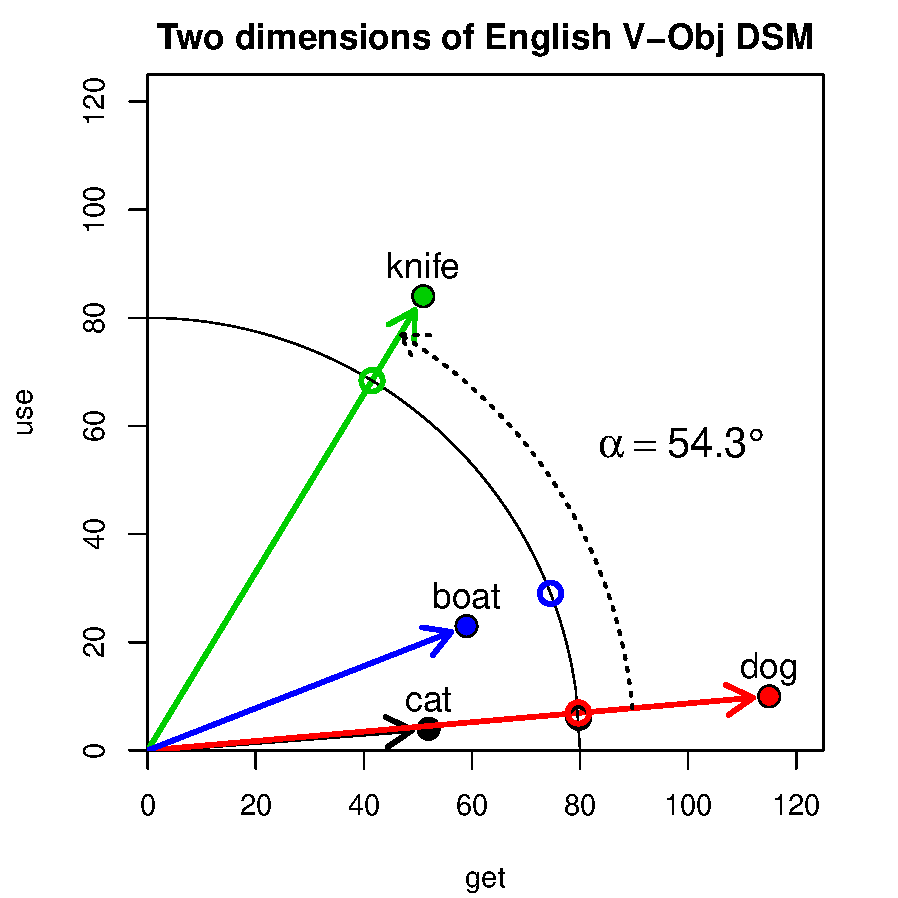
\includegraphics[width=6cm]{img/hieroglyph_2d_5}
    \end{column}
  \end{columns}
\end{frame}

\begin{frame}[fragile]
  \frametitle{Norms and normalization}

\ungap[1]
\begin{Rcode}
> rowNorms(TT$S, method="euclidean")\begin{Rout}
   cat    dog animal   time reason  cause effect 
  6.90   8.96   8.82  10.29   8.13   6.86   6.52 
\end{Rout}
\end{Rcode} %$ de-confuse Emacs

\begin{Rcode}
> TT <- dsm.score(TT, score="freq", transform="log",
                  normalize=TRUE, method="euclidean")
> rowNorms(TT$S, method="euclidean") \REM{all = 1 now}
> dist.matrix(TT, method="euclidean")\begin{Rout}
         cat   dog animal  time reason cause effect
cat    0.000 0.224  0.473 0.782  1.121 1.239  1.161
dog    0.224 0.000  0.398 0.698  1.065 1.179  1.113
animal 0.473 0.398  0.000 0.426  0.841 0.971  0.860
time   0.782 0.698  0.426 0.000  0.475 0.585  0.502
reason 1.121 1.065  0.841 0.475  0.000 0.277  0.198
cause  1.239 1.179  0.971 0.585  0.277 0.000  0.224
effect 1.161 1.113  0.860 0.502  0.198 0.224  0.000\end{Rout}
\end{Rcode} %$ de-confuse Emacs
\end{frame}


\begin{frame}
  \frametitle{Other distance measures}
  % \framesubtitle{}
  
  \begin{itemize}
  \item Information theory: \h{Kullback-Leibler} (KL) \h{divergence} for probability vectors (\hand\ non-negative, $\norm[1]{\vx} = 1$)
    \[
    \KL{\vu}{\vv} = \sum_{i=1}^n u_i \cdot \log_2 \frac{u_i}{v_i}
    \]
    \pause
  \item Properties of KL divergence
    \begin{itemize}
    \item most appropriate in a probabilistic interpretation of $\mathbf{M}$
    \item zeroes in $\vv$ without corresponding zeroes in $\vu$ are problematic
    \item not symmetric, unlike geometric distance measures
    \item alternatives: skew divergence, Jensen-Shannon divergence
    \item[]
    \end{itemize}
    \pause
  \item A symmetric distance measure \citep{Endres:Schindelin:03}
    \[
    D_{\vu\vv} = \KL{\vu}{\vz} + \KL{\vv}{\vz} \quad \text{with} \quad \vz = \frac{\vu + \vv}{2}
    \]
  \end{itemize}
\end{frame}

\begin{frame}
  \frametitle{Similarity measures}
  % \framesubtitle{}
  
  \begin{columns}[c]
    \begin{column}{5cm}
      \begin{itemize}
        \item Angle $\alpha$ between vectors $\vu,\vv\in \setR^n$ is given by
          \begin{align*}
            \cos \alpha &= 
            \frac{\sum_{i=1}^n u_i\cdot v_i}{
              \sqrt{\sum_i u_i^2}\cdot \sqrt{\sum_i v_i^2}}
            \\
            &= \frac{\vu^T \vv}{\norm[2]{\vu}\cdot \norm[2]{\vv}}
        \end{align*}
      \item<2-> \h{cosine} measure of similarity: $\cos \alpha$
        \begin{itemize}
        \item $\cos \alpha = 1$ \so collinear
        \item $\cos \alpha = 0$ \so orthogonal
        \end{itemize}
      \item<2-> Corresponding metric: angular distance $\alpha$
      \end{itemize}
    \end{column}
    \begin{column}{6cm}
      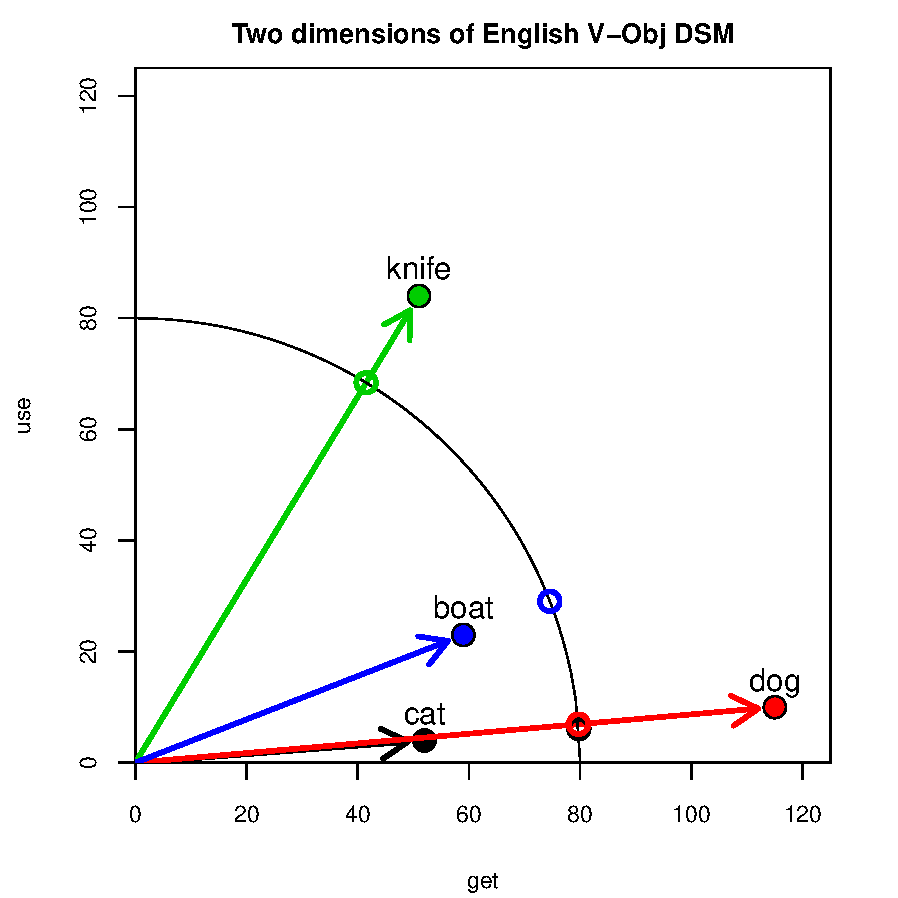
\includegraphics[width=6cm]{img/hieroglyph_2d_4}
    \end{column}
  \end{columns}
\end{frame}

%%%%%%%%%%%%%%%%%%%%%%%%%%%%%%%%%%%%%%%%%%%%%%%%%%%%%%%%%%%%%%%%%%%%%%
\againframe<beamer:8| handout:8>{DSM_parameters}

\begin{frame}
  \frametitle{Dimensionality reduction = model compression}
  % \framesubtitle{}

  \begin{itemize}
  \item Co-occurrence matrix $\mathbf{M}$ is often unmanageably large\\
    and can be extremely sparse
    \begin{itemize}
    \item Google Web1T5: 1M $\times$ 1M matrix with one trillion
      cells, of which less than 0.05\% contain nonzero counts \citep{Evert:10a}
    \end{itemize}
  \item[\So] Compress matrix by reducing dimensionality (= rows)
    \begin{itemize}
    \item[]\pause
    \end{itemize}
  \item \h{Feature selection}: columns with high frequency \& variance
    \begin{itemize}
    \item measured by entropy, chi-squared test, nonzero count, \ldots
    \item may select similar dimensions and discard valuable information
    \item joint selection of multiple features is useful but expensive
    \end{itemize}
    \pause
  \item \h{Projection} into (linear) subspace
    \begin{itemize}
    \item principal component analysis (PCA)
    \item independent component analysis (ICA)
    \item random indexing (RI)
    \item[\hand] intuition: preserve distances between data points
    \end{itemize}
  \end{itemize}
\end{frame}

\begin{frame}
  \frametitle{Dimensionality reduction \& latent dimensions}
  %% \framesubtitle{}

  \citet{Landauer:Dumais:97} claim that LSA dimensionality reduction (and related PCA technique) uncovers \h{latent dimensions} by exploiting correlations between features.

  \begin{columns}
    \begin{column}{6.5cm}
      \begin{itemize}
      \item Example: term-term matrix
      \item V-Obj cooc's extracted from BNC
        \begin{itemize}
        \item targets = noun lemmas\\
        \item features = verb lemmas
        \end{itemize}
      \item feature scaling: association scores (modified $\log$ Dice
        coefficient)
      \item $k=111$ nouns with $f \geq 20$\\
        (must have non-zero row vectors)
      \item $n=2$ dimensions: \emph{buy} and \emph{sell}
      \end{itemize}
    \end{column}
    \begin{column}{4cm}
      \begin{center}\footnotesize
        \begin{tabular}{l|rr}
          noun & \emph{buy} & \emph{sell} \\
          \hline
          \emph{bond}      &  0.28 &  0.77\\
          \emph{cigarette} & -0.52 &  0.44\\
          \emph{dress}     &  0.51 & -1.30\\
          \emph{freehold}  & -0.01 & -0.08\\
          \emph{land}      &  1.13 &  1.54\\
          \emph{number}    & -1.05 & -1.02\\
          \emph{per}       & -0.35 & -0.16\\
          \emph{pub}       & -0.08 & -1.30\\
          \emph{share}     &  1.92 &  1.99\\
          \emph{system}    & -1.63 & -0.70
        \end{tabular}
      \end{center}
    \end{column}
  \end{columns}
\end{frame}

\begin{frame}[c]
  \frametitle{Dimensionality reduction \& latent dimensions}
  %% \framesubtitle{}
  \begin{center}
    \ungap[1]
    \includegraphics[width=8cm]{img/3_buy_sell_labels_only}
  \end{center}
\end{frame}

\begin{frame}
  \frametitle{Motivating latent dimensions \& subspace projection}
  %% \framesubtitle{}

  \begin{itemize}
  \item The \h{latent property} of being a commodity is ``expressed''
    through associations with several verbs: \emph{sell}, \emph{buy},
    \emph{acquire}, \ldots
  \item Consequence: these DSM dimensions will be \h{correlated}
  \item[]\pause
  \item Identify \h{latent dimension} by looking for strong correlations\\
    (or weaker correlations between large sets of features)%
  \item Projection into subspace $V$ of $k < n$ latent dimensions\\
    as a ``\h{noise reduction}'' technique \so \hh{LSA}
  \item Assumptions of this approach:
    \begin{itemize}
    \item ``latent'' distances in $V$ are semantically meaningful
    \item other ``residual'' dimensions represent chance co-occurrence
      patterns, often particular to the corpus underlying the DSM
    \end{itemize}
  \end{itemize}
\end{frame}

\begin{frame}[c]
  \frametitle{Centering the data set}
  %% \framesubtitle{}

  \begin{columns}[c]
    \begin{column}{40mm}
      \begin{itemize}
      \item \h<beamer:1| handout:1>{Uncentered\\ data set}%
        \gap
      \item \h<beamer:2| handout:2>{Centered\\ data set}%
        \gap
      \item \h<beamer:3| handout:3>{Variance of\\ centered data}%
        \gap
      \end{itemize}
      \visible<beamer:3| handout:3>{%
        \[
        \sigma^2 = \tfrac{1}{k-1} \sum_{i=1}^k \norm{\vx[i]}^2
        \]
      }
    \end{column}
    \begin{column}{60mm}
      \only<beamer:1| handout:1>{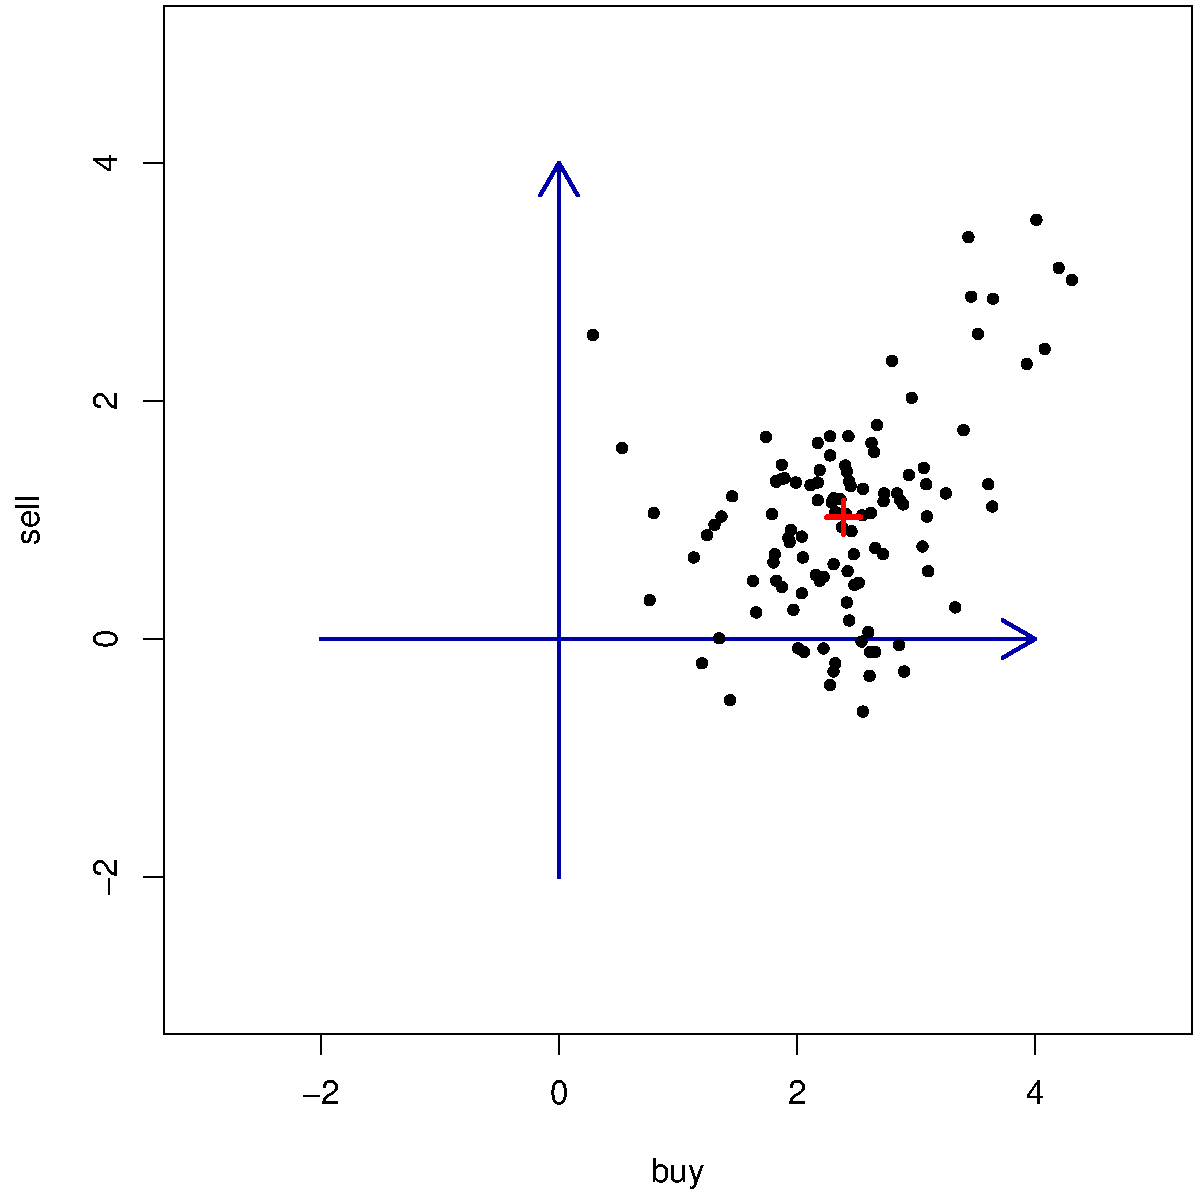
\includegraphics[width=6cm]{img/3_buy_sell_uncentered}}%
      \only<beamer:2| handout:2>{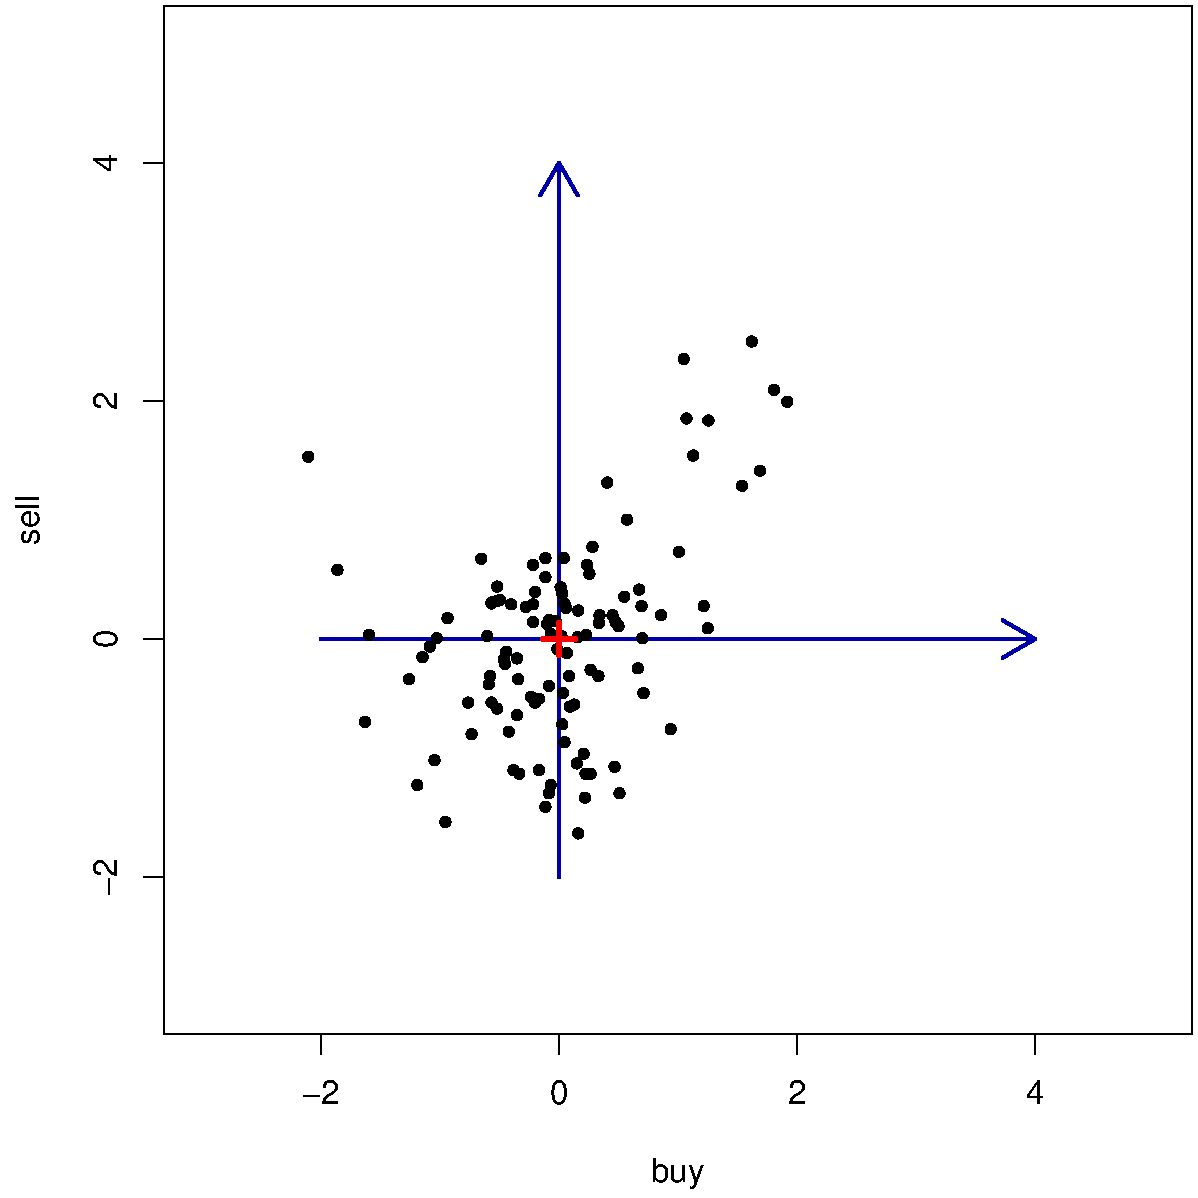
\includegraphics[width=6cm]{img/3_buy_sell_centered}}%
      \only<beamer:3| handout:3>{\includegraphics[width=6cm]{img/3_buy_sell_variance}}%
    \end{column}
  \end{columns}
\end{frame}

\begin{frame}<beamer:1-6| handout:1-3>[c]
  \frametitle{Projection and preserved variance: examples}
  %% \framesubtitle{}

  \begin{center}
    \only<beamer:1| handout:0>{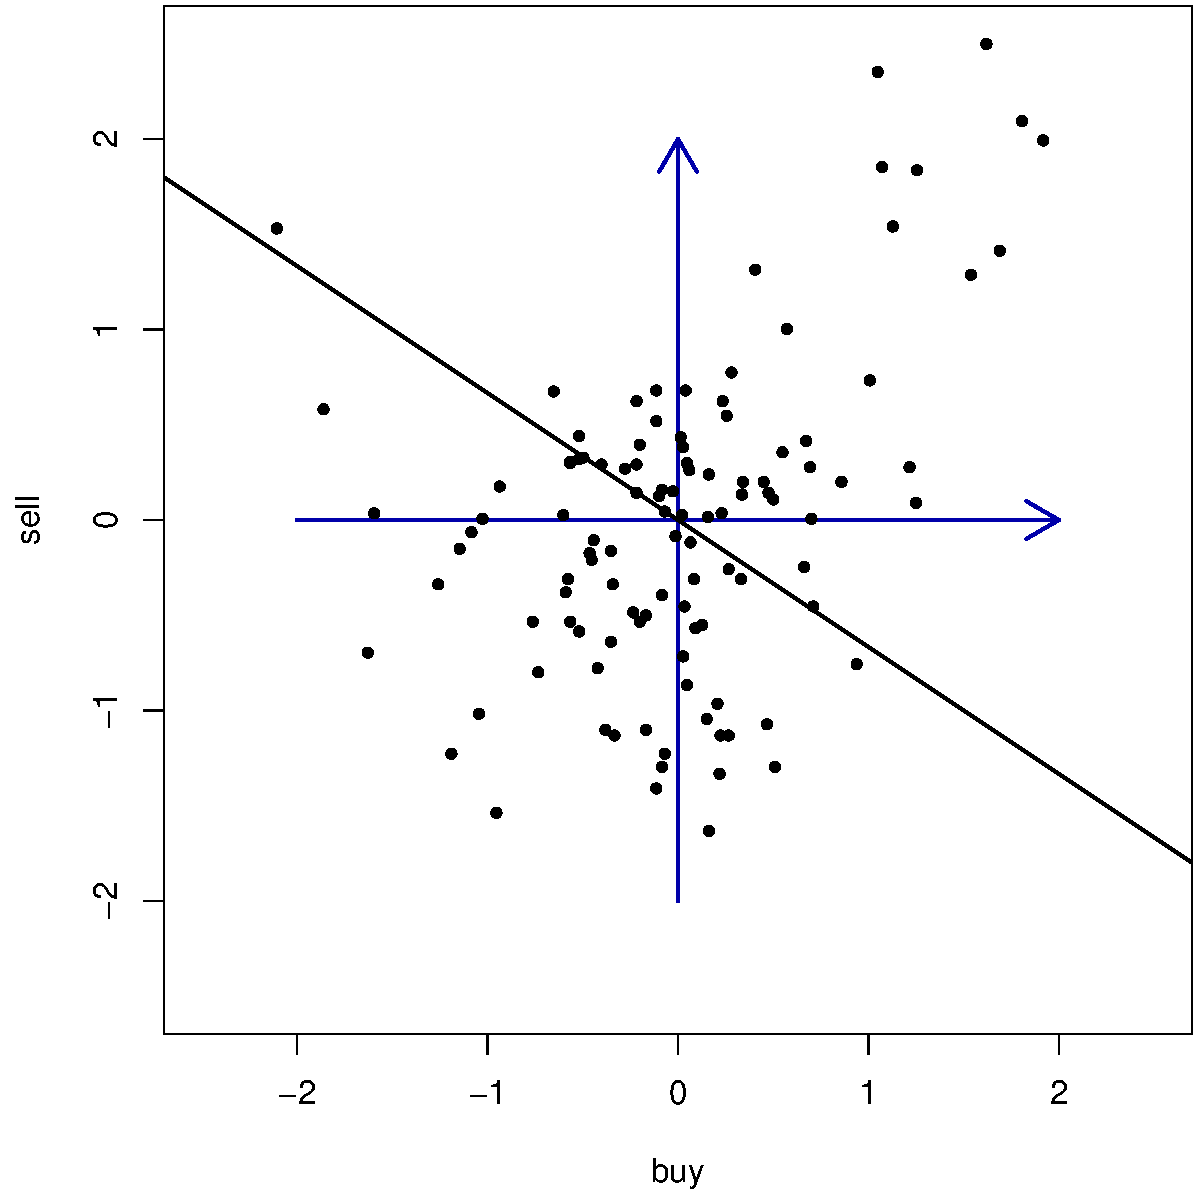
\includegraphics[width=7.5cm]{img/3_buy_sell_1_axis}}%
    \only<beamer:2| handout:1>{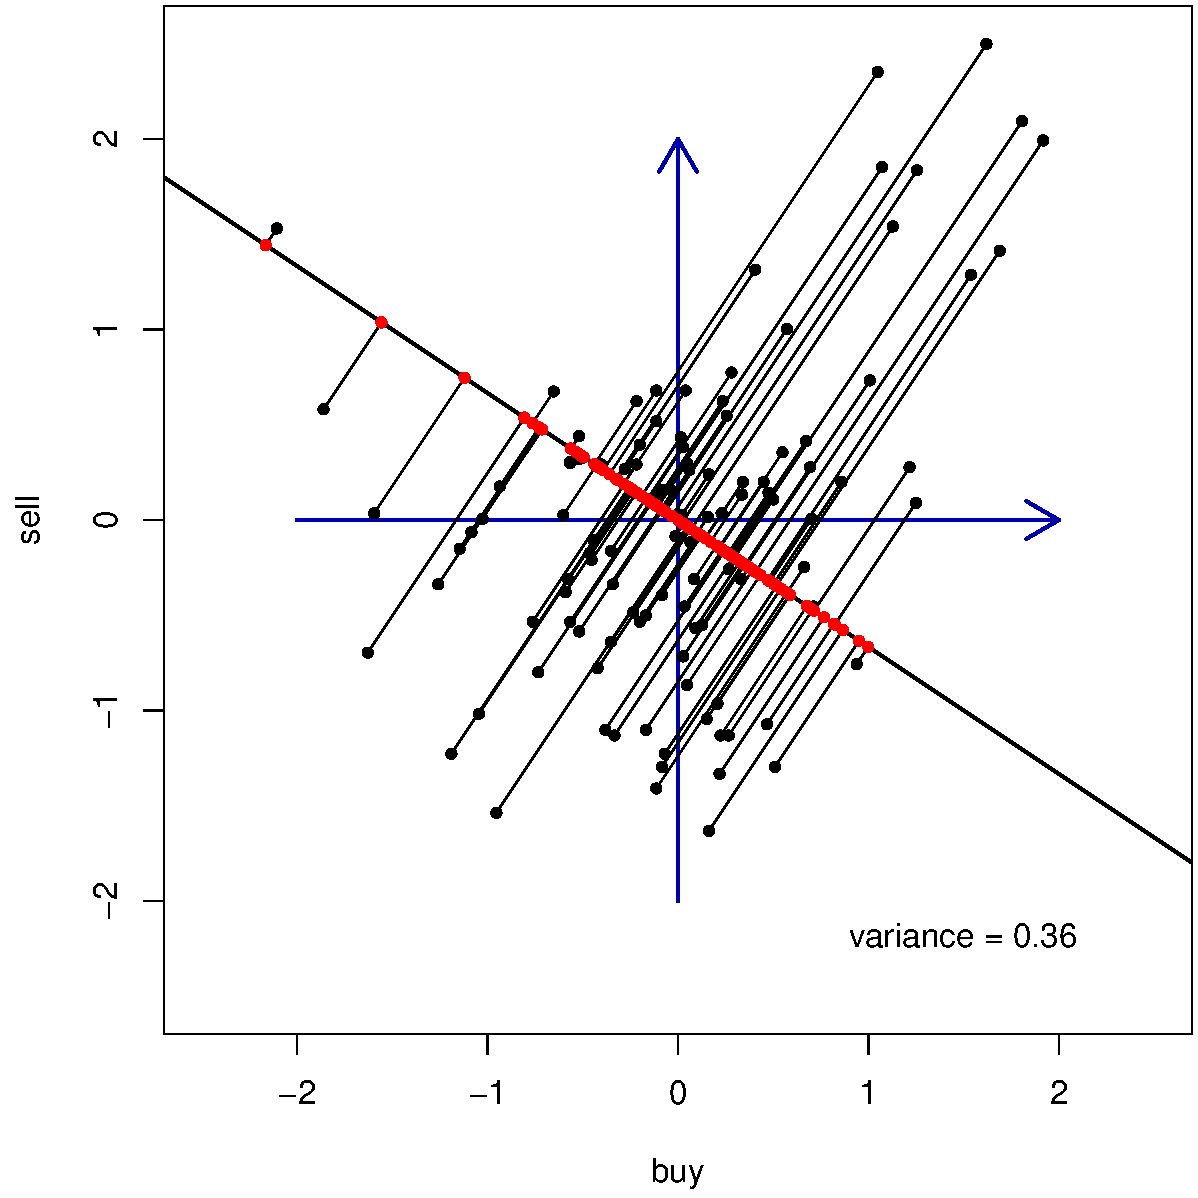
\includegraphics[width=7.5cm]{img/3_buy_sell_1_projection}}%
    \only<beamer:3| handout:0>{\includegraphics[width=7.5cm]{img/3_buy_sell_2_axis}}%
    \only<beamer:4| handout:2>{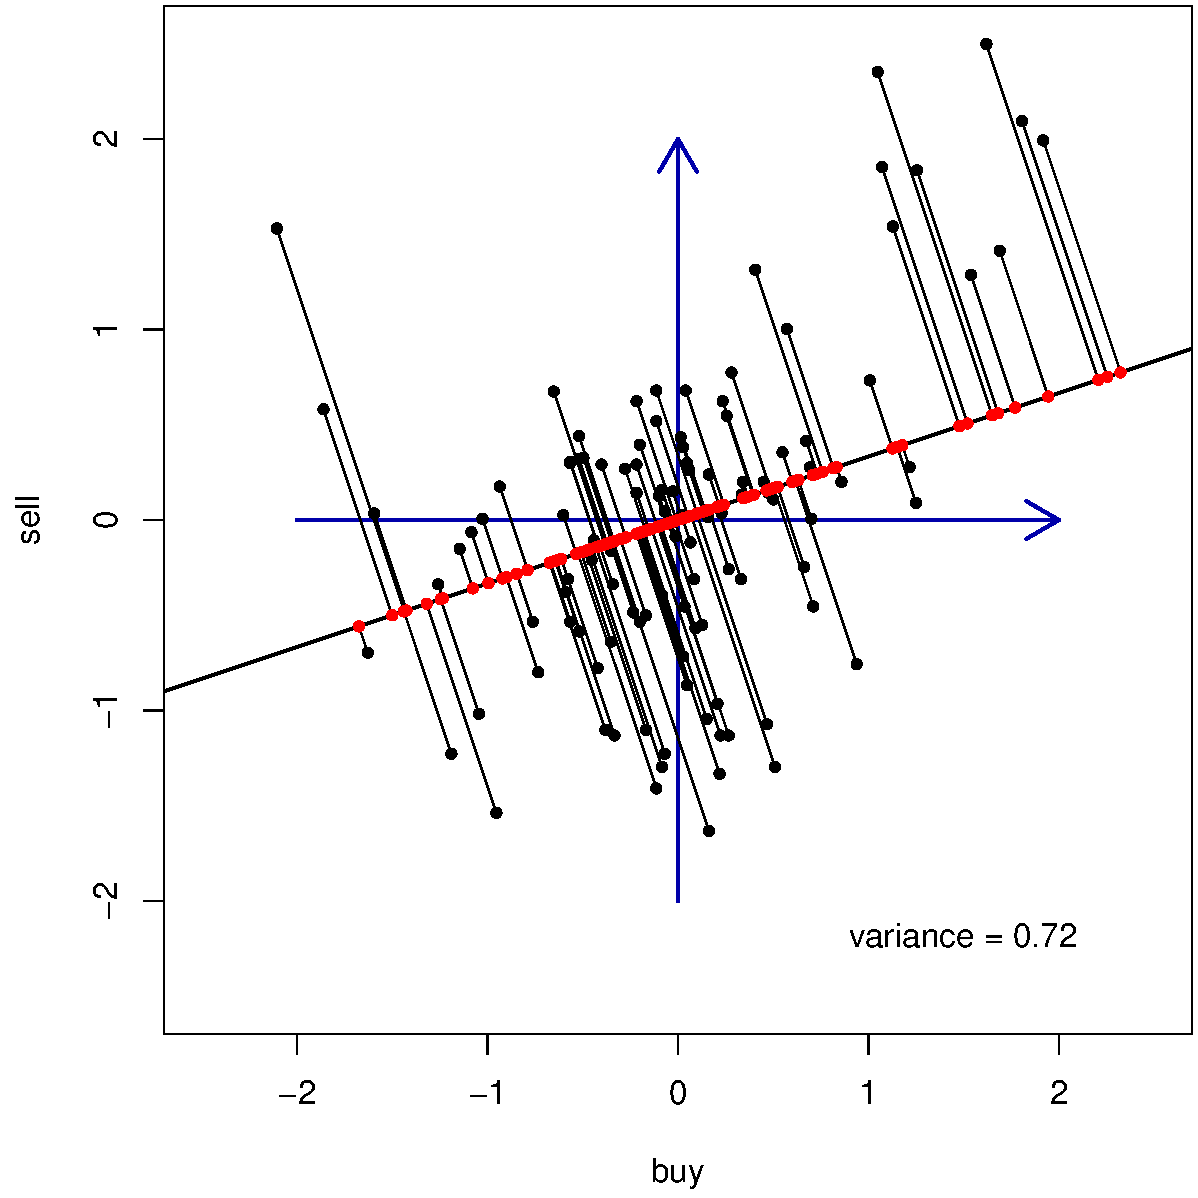
\includegraphics[width=7.5cm]{img/3_buy_sell_2_projection}}%
    \only<beamer:5| handout:0>{\includegraphics[width=7.5cm]{img/3_buy_sell_3_axis}}%
    \only<beamer:6| handout:3>{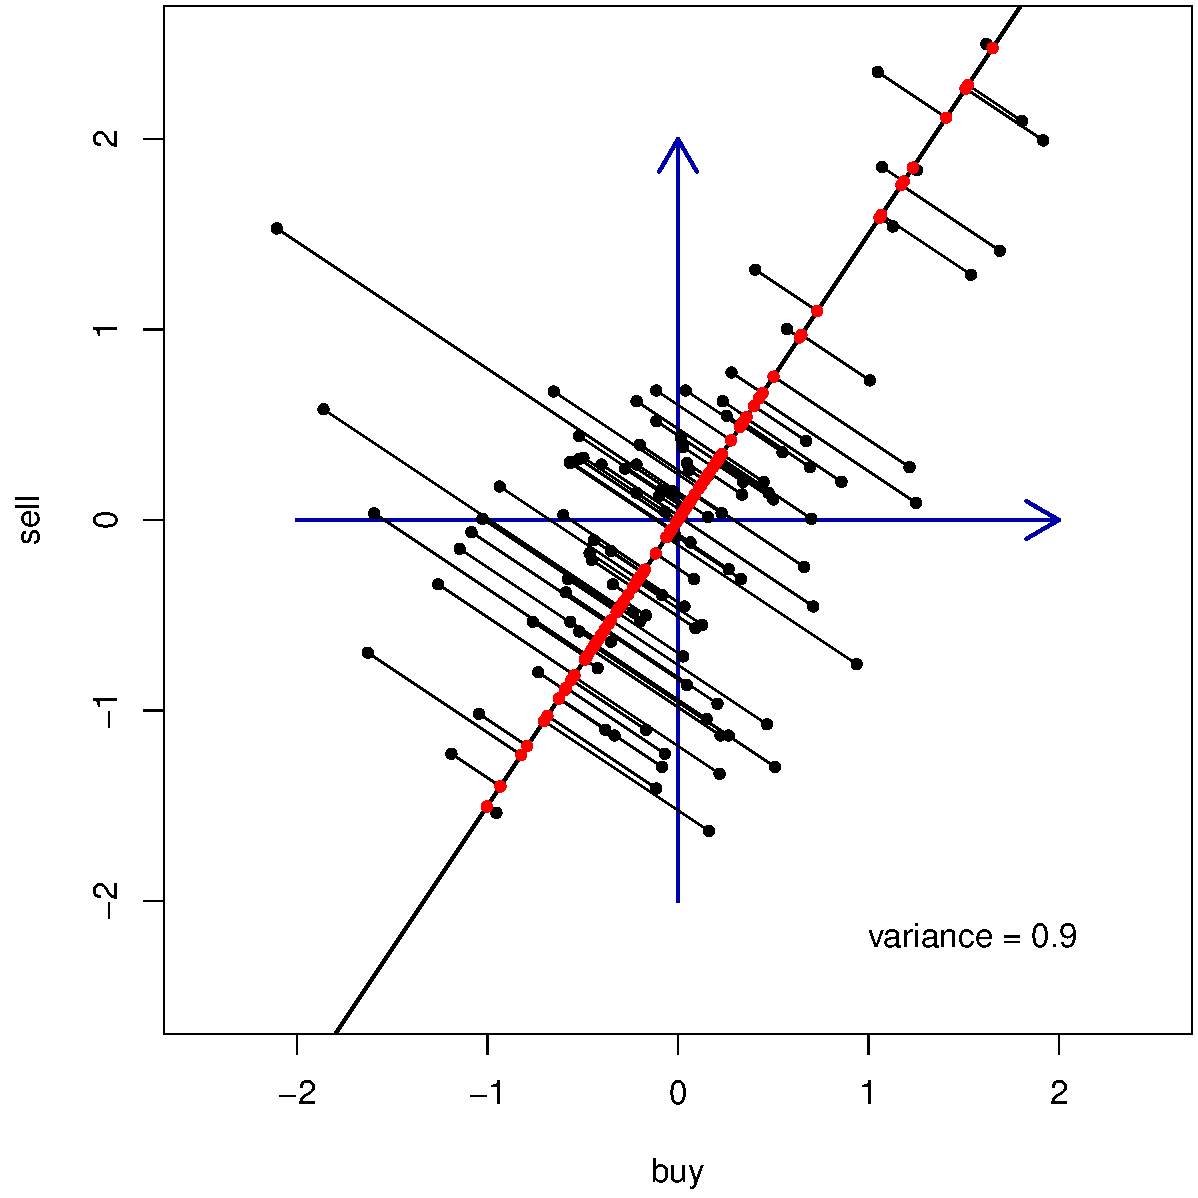
\includegraphics[width=7.5cm]{img/3_buy_sell_3_projection}}%
  \end{center}
\end{frame}


\begin{frame}[c]
  \frametitle{Orthogonal PCA dimensions}
  %% \framesubtitle{}

  \begin{center}
    %% \only<beamer:1| handout:0>{\includegraphics[width=8cm]{img/3_buy_sell_pca}}
    \only<beamer:1| handout:1>{\includegraphics[width=7.5cm]{img/3_buy_sell_pca_labels}}%
  \end{center}
\end{frame}

\begin{frame}[fragile]
  \frametitle{Dimensionality reduction in practice}

\ungap[1.5]
\begin{Rcode}
\REM{it is customary to omit the centring: SVD dimensionality reduction}
> TT2 <- dsm.projection(TT, n=2, method="svd")
> TT2\begin{Rout}
         svd1    svd2
cat    -0.733 -0.6615
dog    -0.782 -0.6110
animal -0.914 -0.3606
time   -0.993  0.0302
reason -0.889  0.4339
cause  -0.817  0.5615
effect -0.871  0.4794
\end{Rout}
> x <- TT2[, 1] \REM{first latent dimension}
> y <- TT2[, 2] \REM{second latent dimension}
> plot(TT2, pch=20, col="red", 
       xlim=extendrange(x), ylim=extendrange(y))
> text(TT2, rownames(TT2), pos=3)    
\end{Rcode}
  
\end{frame}


%%%%%%%%%%%%%%%%%%%%%%%%%%%%%%%%%%%%%%%%%%
\subsection{Examples}

\begin{frame}
  \frametitle{Some well-known DSM examples}

  \ungap
  \begin{block} {Latent Semantic Analysis \citep{Landauer:Dumais:97}}
    \begin{itemize}
    \item term-context matrix with document context
    \item weighting: log term frequency and term entropy
    \item distance measure: cosine
    \item dimensionality reduction: SVD
    \end{itemize}
  \end{block}
  
  \pause
  \begin{block} {Hyperspace Analogue to Language \citep{Lund:Burgess:96}}
    \begin{itemize}
    \item term-term matrix with surface context
    \item structured (left/right) and distance-weighted frequency counts
    \item distance measure: Minkowski metric ($1\leq p \leq 2$)
    \item dimensionality reduction: feature selection (high variance)
    \end{itemize}
  \end{block}
\end{frame}

\begin{frame}
  \frametitle{Some well-known DSM examples}

  \ungap
  \begin{block} {Infomap NLP \citep{Widdows:04}}
    \begin{itemize}
    \item term-term matrix with unstructured surface context
    \item weighting: none
    \item distance measure: cosine
    \item dimensionality reduction: SVD
    \end{itemize}
  \end{block}

  \pause
  \begin{block} {Random Indexing \citep{Karlgren:Sahlgren:01}}
    \begin{itemize}
    \item term-term matrix with unstructured surface context
    \item weighting: various methods 
    \item distance measure: various methods
    \item dimensionality reduction: random indexing (RI)
    \end{itemize}
  \end{block}
\end{frame}

\begin{frame}
  \frametitle{Some well-known DSM examples}

  \ungap
  \begin{block}{Dependency Vectors \citep{Pado:Lapata:07}}
    \begin{itemize}
    \item term-term matrix with unstructured dependency context
    \item weighting: log-likelihood ratio
    \item distance measure: PPMI-weighted Dice \citep{Lin:98b}
    \item dimensionality reduction: none
    \end{itemize}
  \end{block}
  
  \pause
  \begin{block} {Distributional Memory \citep{Baroni:Lenci:10}}
    \begin{itemize}
    \item term-term matrix with structured and unstructered dependencies + knowledge patterns
    \item weighting: local-MI on type frequencies of link patterns
    \item distance measure: cosine
    \item dimensionality reduction: none
    \end{itemize}
  \end{block}
\end{frame}

%%%%%%%%%%%%%%%%%%%%%%%%%%%%%%%%%%%%%%%%%%%%%%%%%%%%%%%%%%%%%%%%%%%%%%
\section{Building a DSM}

%%%%%%%%%%%%%%%%%%%%%%%%%%%%%%%%%%%%%%%%%%%%%%%%%%%%%%%%%%%%%%%%%%%%%%
\subsection{Sparse matrices}

\begin{frame}
  \frametitle{Scaling up to the real world}
  %% \framesubtitle{}

  \begin{itemize}
  \item So far, we have worked on minuscule \hh{toy models}
  \item[\hand] We want to scale up to \h{real world} data sets now
    \begin{itemize}
    \item[]
    \end{itemize}
  \item<2-> Example 1: window-based DSM on BNC content words
    \begin{itemize}
    \item 83,926 lemma types with $f\geq 10$
    \item term-term matrix with 83,926 $\cdot$ 83,926 = 7 billion entries
    \item standard representation requires 56 GB of RAM (8-byte floats)%
    \item only 22.1 million non-zero entries ($= 0.32\%$)
    \item[]
    \end{itemize}
  \item<3-> Example 2: Google Web 1T 5-grams (1 trillion words)
    \begin{itemize}
    \item more than 1 million word types with $f\geq 2500$
    \item term-term matrix with 1 trillion entries requires 8 TB RAM
    \item only 400 million non-zero entries ($= 0.04\%$)
    \end{itemize}
  \end{itemize}
\end{frame}

\begin{frame}
  \frametitle{Sparse matrix representation}
  %% \framesubtitle{}

  \ungap
  \begin{itemize}
  \item Invented example of a \hh{sparsely populated} DSM matrix
    \begin{center}\footnotesize
      \begin{tabular}{r | cccccc}
        & eat & get & hear & kill & see & use \\
        \midrule
        boat  &   $\cdot$  & 59  &   $\cdot$  &   $\cdot$  & 39 &  23 \\
        cat   &   $\cdot$  &  $\cdot$  &   $\cdot$  &  26  & 58 &   $\cdot$ \\
        cup   &   $\cdot$  & 98  &   $\cdot$  &   $\cdot$  &  $\cdot$ &   $\cdot$ \\
        dog   &  33  &  $\cdot$  &  42  &   $\cdot$  & 83 &   $\cdot$ \\
        knife &   $\cdot$  &  $\cdot$  &   $\cdot$  &   $\cdot$  &  $\cdot$ &  84 \\
        pig   &   9  &  $\cdot$  &   $\cdot$  &  27  &  $\cdot$ &   $\cdot$ 
      \end{tabular}
    \end{center}
    \gap\pause
  \item Store only non-zero entries in compact \h{sparse matrix format}
    \begin{center}\footnotesize
      \begin{tabular}{r|r|r c r|r|r}
        row & col & value && row & col & value \\
        \cline{1-3} \cline{5-7}
        1  &  2  &  59 &&  4  &  1  &  33 \\
        1  &  5  &  39 &&  4  &  3  &  42 \\
        1  &  6  &  23 &&  4  &  5  &  83 \\
        2  &  4  &  26 &&  5  &  6  &  84 \\
        2  &  5  &  58 &&  6  &  1  &   9 \\
        3  &  2  &  98 &&  6  &  4  &  27 \\
       \end{tabular}
    \end{center}
  \end{itemize}
\end{frame}

\begin{frame}
  \frametitle{Working with sparse matrices}
  %% \framesubtitle{}

  \begin{itemize}
  \item Compressed format: each row index (or column index) stored only once,
    followed by non-zero entries in this row (or column)%
    \begin{itemize}
    \item convention: \h{column-major} matrix (data stored by columns)
    \item[]
    \end{itemize}
  \item Specialised algorithms for sparse matrix algebra
    \begin{itemize}
    \item especially matrix multiplication, solving linear systems, etc.
    \item take care to avoid operations that create a dense matrix!
    \item[]
    \end{itemize}
  \item<2-> \hh{R} implementation: \texttt{Matrix} package
    \begin{itemize}
    \item essential for real-life distributional semantics
    \item \texttt{wordspace} provides additional support for sparse matrices (vector distances, sparse SVD, \ldots)
    \item[]
    \end{itemize}
  \item<2-> Other software: Matlab, Octave, Python + SciPy
  \end{itemize}
\end{frame}

%%%%%%%%%%%%%%%%%%%%%%%%%%%%%%%%%%%%%%%%%%%%%%%%%%%%%%%%%%%%%%%%%%%%%%
\subsection{Example: a verb-object DSM}

\begin{frame}[fragile]
  \frametitle{Triplet tables}

  \ungap[1]
  \begin{itemize}
  \item A sparse DSM matrix can be represented as a table of triplets (target, feature, co-occurrence frequency)
    \begin{itemize}
    \item for syntactic co-occurrence and term-document matrices, marginals can be computed from a complete triplet table
    \item for surface and textual co-occurrence, marginals have to be provided in separate files (see \code{?read.dsm.triplet})
    \end{itemize}
  \end{itemize}
  
  \begin{center}\footnotesize
    \begin{tabular}{>{\color{primary}}ll>{\color{primary}}l>{\color{primary}}rr}
    \toprule
    noun & rel & verb   &  f &    mode \\ 
    \midrule
    dog & subj & bite   &  3 &  spoken \\ 
    dog & subj & bite   & 12 & written \\ 
    dog &  obj & bite   &  4 & written \\ 
    dog &  obj & stroke &  3 & written \\
    \ldots &  \ldots & \ldots  & \ldots & \ldots \\ 
    \bottomrule
    \end{tabular}
  \end{center}
  
  \begin{itemize}
  \item \code{\small DSM\_VerbNounTriples\_BNC} contains additional information
    \begin{itemize}
    \item syntactic relation between noun and verb
    \item written or spoken part of the British National Corpus
    \end{itemize}
  \end{itemize}

\end{frame}

\begin{frame}[fragile]
  \frametitle{Constructing a DSM from a triplet table}

  \begin{itemize}
  \item Additional information can be used for filtering (verb-object relation), or aggregate frequencies (spoken + written BNC)
  \end{itemize}

\ungap[.5]
\begin{Rcode}
> tri <- subset(DSM_VerbNounTriples_BNC, rel == "obj")
\end{Rcode}

  \begin{itemize}
  \item Construct DSM object from triplet input
    \begin{itemize}
    \item \code{raw.freq=TRUE} indicates raw co-occurrence frequencies (rather than a pre-weighted DSM)
    \item constructor aggregates counts from duplicate entries
    \item marginal frequencies are automatically computed
    \end{itemize}
  \end{itemize}

\ungap[.5]
\begin{Rcode}
> VObj <- dsm(target=tri$noun, feature=tri$verb, 
              score=tri$f, raw.freq=TRUE)
> VObj \REM{inspect marginal frequencies (e.g.\ head(VObj$rows, 20))}
\end{Rcode}
\end{frame}

\begin{frame}[fragile]
  \frametitle{Exploring the DSM}

\begin{Rcode}
> VObj <- dsm.score(VObj, score="MI", normalize=TRUE)

> nearest.neighbours(VObj, "dog") \REM{angular distance}\begin{Rout}
   horse      cat   animal   rabbit     fish      guy  
    73.9     75.9     76.2     77.0     77.2     78.5  
 cichlid      kid      bee creature 
    78.6     79.0     79.1     79.5 
\end{Rout}
> nearest.neighbours(VObj, "dog", method="manhattan")
\REM{NB: we used an incompatible Euclidean normalization!}

> VObj50 <- dsm.projection(VObj, n=50, method="svd")
> nearest.neighbours(VObj50, "dog")
\end{Rcode}
\end{frame}



%%%%%%%%%%%%%%%%%%%%%%%%%%%%%%%%%%%%%%%%%%%%%%%%%%%%%%%%%%%%%%%%%%%%%%
%% References (if any)

\frame[allowframebreaks]{
  \frametitle{References}
  \bibliographystyle{natbib-stefan}
  \begin{scriptsize}
    \bibliography{dsm}
  \end{scriptsize}
}

\end{document}
